% % Full page illustration
% \begin{figure}[!hbtp]
%     \centering
%     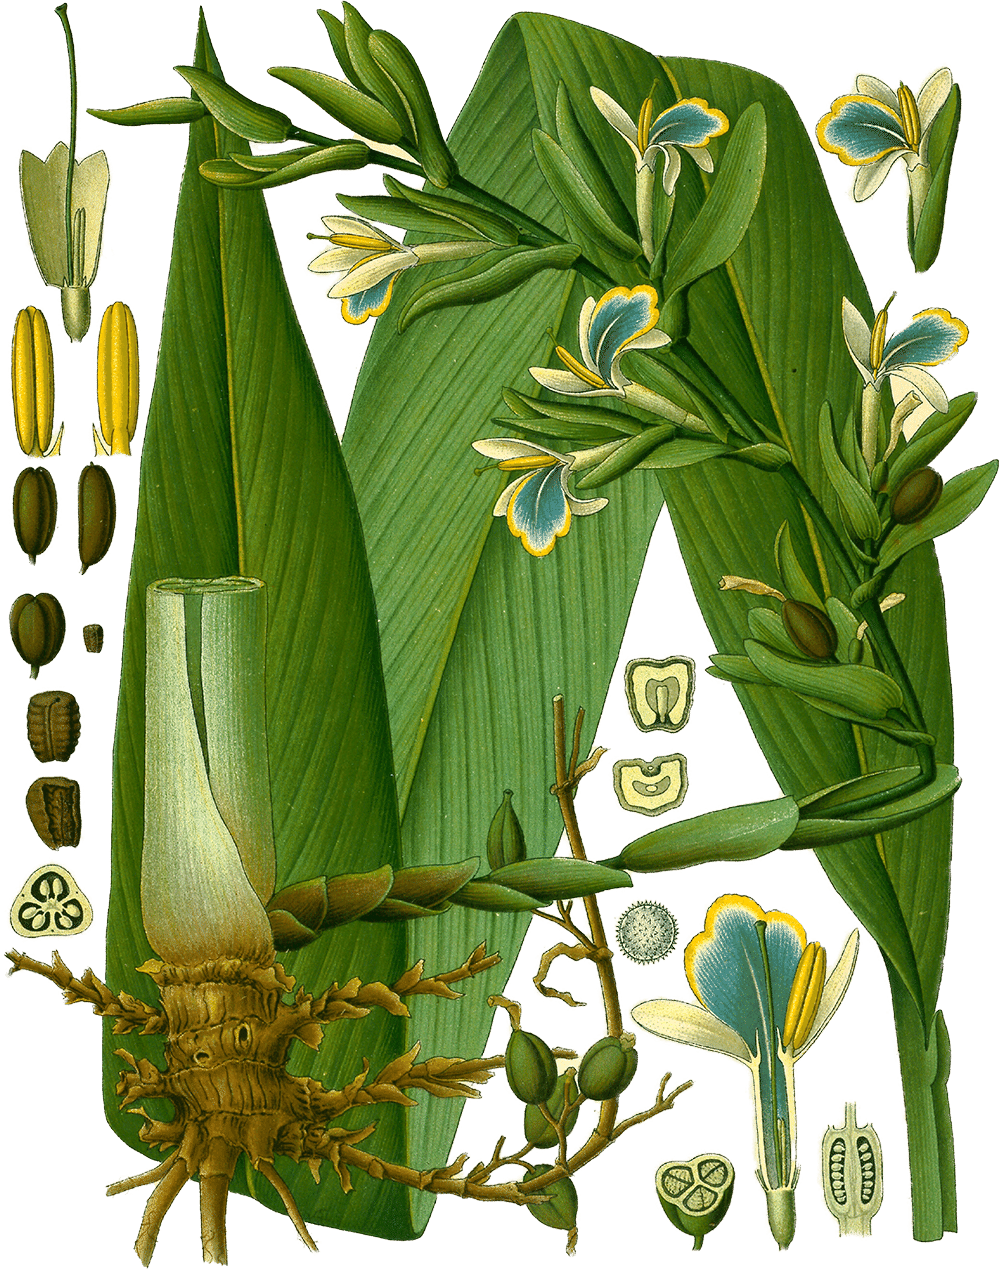
\includegraphics[width=\textwidth]{imgs/kohler/cardamom_kohler_min.png}
%     \caption{\taxonn{Cinnamomum verum}{J.Presl.} (syn. \taxonn{C. zeylanicum}{Blume}), the cinnamon tree in Köhler's Medicinal Plants \pvolcite[]{1}[78]{kohler_kohlers_1887}.}
%     \label{fig:kohler_cinnamon}
% \end{figure}



\section{Cinnamon \& Cassia}
\label{sec:cinnamon}
\label{sec:cassia}

\begin{spice}\label{spice:cinnamon}
\textsc{Cinnamon} \hfill \href{https://powo.science.kew.org/taxon/463752-1}{POWO} \\
\textbf{English:} \textit{cinnamon}. 
\textbf{Arabic:} {\arabicfont{قرفة}} \textit{qirfa} [rind; bark]; {دارصيني} \textit{dārsīnī}. 
\textbf{Chinese:} {\tc{錫蘭肉桂}} \textit{xīlánròuguì} [Ceylon-flesh-cinnamon]. 
\textbf{Hungarian:} \textit{fahéj} [tree-bark].  \\
\noindent{\color{black}\rule[0.5ex]{\linewidth}{.5pt}}
\begin{tabular}{@{}p{0.25\linewidth}@{}p{0.75\linewidth}@{}}
Plant species: & \taxonn{Cinnamomum verum}{J.Presl.} (syn. \taxonn{Cinnamomum zeylanicum}{Blume}) \\
Family: & \textit{Lauraceae} \\
part used: & bark; leaf \\
Region of origin: & Sri Lanka; SW. India \\
Cultivated in: & Sri Lanka; Seychelles; Madagascar; India \\
Color: & warm yellowish-brown, cinnamon \sample{cinnamon} \\
\end{tabular}
\end{spice}

\begin{figure}[!ht]
	\vspace{-4ex}
	\centering
	\subfloat[quills]{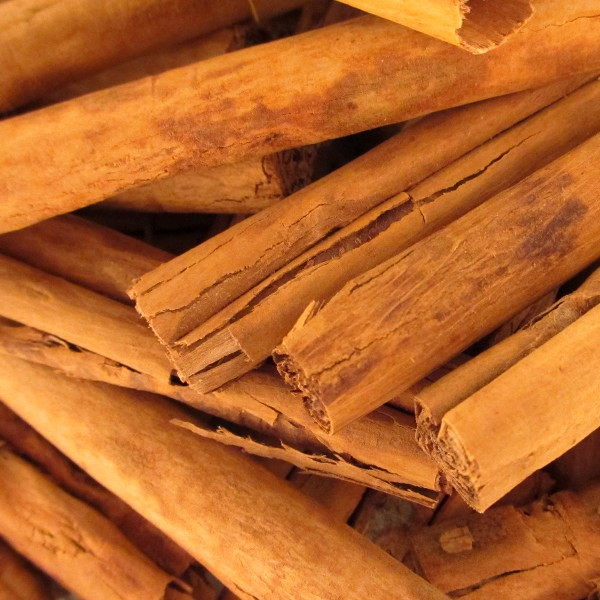
\includegraphics[width=0.3\linewidth]{imgs/spices/cinnamon-1.jpg}}
	\hfill
	\subfloat[quills]{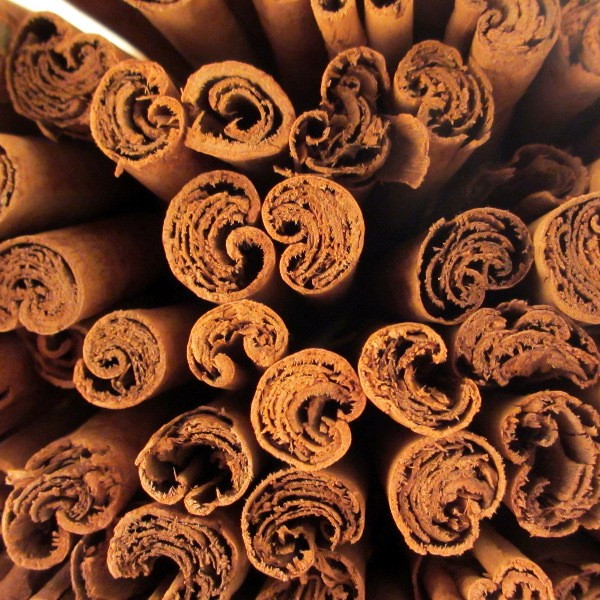
\includegraphics[width=0.3\linewidth]{imgs/spices/cinnamon-2.jpg}}
	\hfill
	\subfloat[leaves]{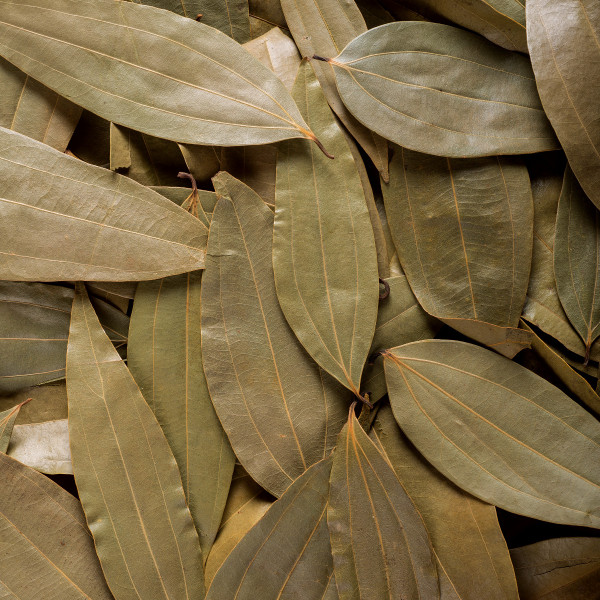
\includegraphics[width=0.3\linewidth]{imgs/spices/cinnamon-4.jpg}}
	\caption{Cinnamon quills, powder, and leaves from \textit{Cinnamomum verum}.}
	\label{fig:cinnamon_imgs}
\end{figure}

Cinnamon is well-known around the world for its sweet aroma and flavor, and as one of the oldest spices of commerce. It was a sought-after substance in rituals and traditional medicine systems of different cultures, and today it is an essential spice of several cuisines---both Eastern and Western. Cinnamon has maintained its level of demand ever since humans first traded it, and even in contemporary times it is the second most important spice in the markets of Europe and the United States (including cassia cinnamon), falling only behind black pepper \parencite[]{ravindran_cinnamon_2004}.

Cinnamon comes from the inner bark (cortex) of the tropical tree \taxonn{Cinnamomum verum}{J.Presl} (syn. \taxonn{C. zeylanicum}{Blume})\footnote{It is difficult to navigate between the hundreds of species and subspecies of cinnamon and their overlapping botanical taxons and binomial synonyms, \textit{C. verum} for example has 51 scientific synonyms, mainly a result of botanical history and competing naturalists. In plant taxonomy, species often have dozens of scientific names called ``synonyms''. If there is consensus on the name within the scientific community, that binomial name (appended with the abbreviated name of the person who coined it) will be marked as ``accepted'', while the status of the other names will be ``synonym'', or ``unresolved''. This is the product of the efforts of the last couple hundred years, when botanists tried to collect, describe, name, and categorize plant life around the world. As the consensus changes with time, competing names can appear in the literature. Botanical databases, such as the \gls{WFO} and \gls{POWO}, or specialized plant name checklists usually list all synonyms of a species to help us orientate in the jungle of plant nomenclature. Synonyms (abbreviated as syn.) are only given if a plant is known by multiple names in non-specialist literature, such as the case above.}, which are stripped and rolled into quills of several tightly packed layers by skilled peelers of (mostly) Sri Lanka, where the plant is native. In a rare example, the literal translations of the binomial names \textit{C. verum} meaning `true cinnamon', and \textit{C. zeylanicum} meaning `Ceylon cinnamon'\footnote{Ceylon is the former name of Sri Lanka} are used as common names for cinnamon in several languages. 

% etymology of Ceylon/serendipity

\begin{spice}\label{spice:cassia}
\textsc{Cassia} \hfill \href{https://powo.science.kew.org/taxon/463288-1}{POWO} \\
\textbf{English:} \textit{cassia}. 
\textbf{Arabic:} {\arabicfont{سليخة}} \textit{salīkha} [peel; bark]. 
\textbf{Chinese:} {\traditionalchinesefont{肉桂}} \textit{ròuguì} [flesh-cinnamon]. 
\textbf{Hungarian:} \textit{kasszia(fahéj)} [cassia (tree-bark)].  \\
\noindent{\color{black}\rule[0.5ex]{\linewidth}{.5pt}}
\begin{tabular}{@{}p{0.25\linewidth}@{}p{0.75\linewidth}@{}}
Plant species: & \taxonn{Cinnamomum cassia}{(L.) J.Presl.} (syn. \taxonn{Cinnamomum aromaticum}{Nees}); \textit{et al.} \\
Family: & \textit{Lauraceae} \\
part used: & bark; fruit \\
Region of origin: & nan \\
Cultivated in: & Indonesia; China; Vietnam; Timor-Leste; etc. \\
Color: & reddish brown \\
\end{tabular}
\end{spice}

\begin{figure}[!ht]
	\vspace{-4ex}
	\centering
	\subfloat[stick]{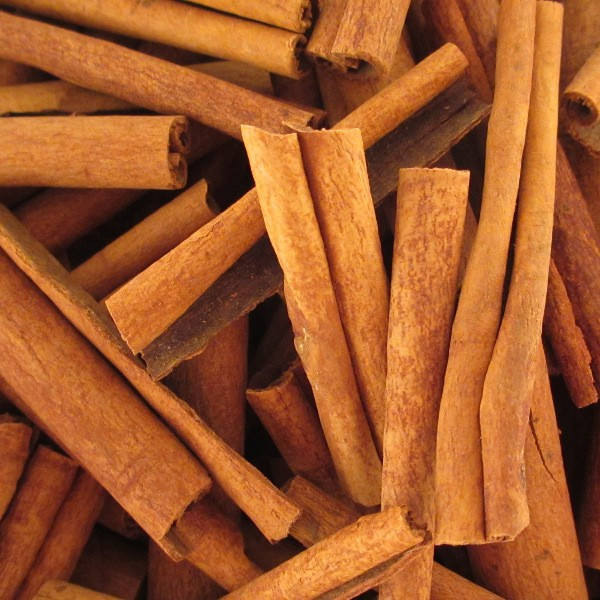
\includegraphics[width=0.3\linewidth]{imgs/spices/cassia-1.jpg}}
	\hfill
	\subfloat[powder]{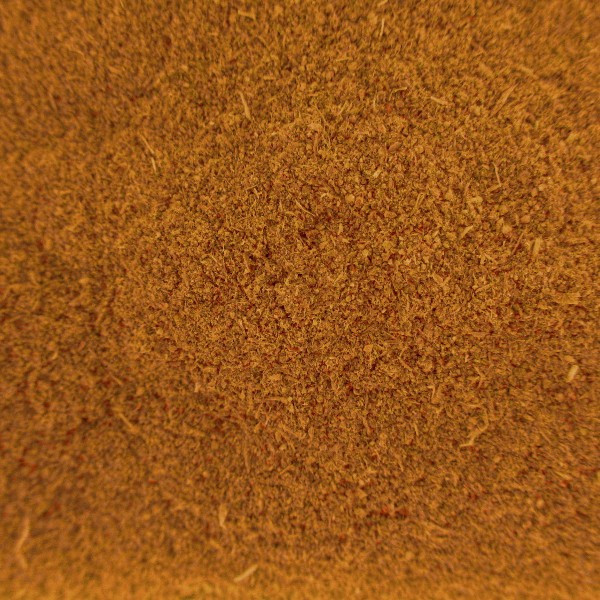
\includegraphics[width=0.3\linewidth]{imgs/spices/cinnamon-3.jpg}}
	\hfill
	\subfloat[buds (dried unripe fruits)]{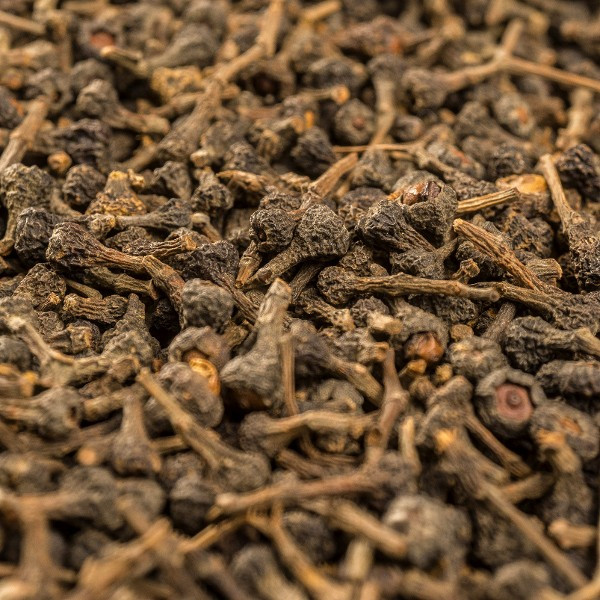
\includegraphics[width=0.3\linewidth]{imgs/spices/cassia-2.jpg}}
	\caption{Cassia sticks and ``buds'' from \textit{Cinnamomum cassia}.}
	\label{fig:cassia_imgs}
\end{figure}

The phrase \textit{true cinnamon} implies that there is a false cinnamon as well, and that would be cassia. Cassia, also knows as Chinese cinnamon, Chinese cassia, cassia cinnamon, and---somewhat harshly---bastard cinnamon, is obtained similarly from the aromatic inner barks of closely related species, especially \taxonn{Cinnamomum cassia}{(L.) J.Presl.} (syn. \taxonn{C. aromaticum}{Nees}), which is produced in Southeast China and Vietnam. Although seemingly very similar to the uninitiated eye, the two spices are different in many ways. Cassia is more hard and coarse, it is made up of a single layer of thicker rind that have curled up in the heat of the day after harvesting, in the shape of a scroll. This is the cinnamon stick that most of us are familiar with, and it is capable to damage a home grinder. It is also a bit more darker reddish brown in color, and more pungent in flavor. Ceylon cinnamon on the other hand is more fragile, slightly pale in color, and supposedly more delicate in taste because it offers a combination of different essential oils besides cinnamaldehyde (the principal component responsible for its aroma and flavor). Both are marketed in powdered form as well, and as such they are indistinguishable; creating room for adulteration. Since the Europeans took over the cinnamon trade of Sri Lanka and tapping the source of ``true cinnamon'' (first by the Portuguese, who got a foothold in the city of Colombo in 1518 together with trading concessions), there is a still ongoing notion that cassia is an inferior product \parencite{chennault_reclusive_2006}. And this belief eventually became reflected on the plant's Linnaean name. A few cuisines also make use of the leaves (usually from \textit{C. verum}), and the dried, immature fruits called cinnamon buds (usually from \textit{C. cassia}).

% French \textit{baies de cannelier}

There are a handful of other species that are cultivated as a source of commercial cassia, such as \textit{C. burmannii} (Indonesian cassia/cinnamon, Padang cassia, Batavia cassia, Korintje (cassia)), \textit{C. loureiroi} (Vietnamese cassia/cinnamon, Saigon cinnamon), and \textit{C. tamala} (Indian cassia (lignea), Indian bark, Malabathri bark), which is more know for its leaf as Indian bay leaf, malabathrum, or tejpat. As reported in \textcite[10]{ravindran_cinnamon_2004}, \textit{C. loureiroi} is extremely rare, and in actuality most of what is known as Vietnamese cassia or Saigon cinnamon is in fact \textit{C. cassia}, contrary to what is claimed in most of the literature. This is supported by reports from botanists of French Indochina who insisted that Saigon cinnamon is brought from the north by Chinese and Annamese merchants \parencite[400]{hu_food_2005}. \textcite{hu_food_2005} recounts us a personal experience from the 1960s, regarding a professor of pharmacy asking assistance in the identification of a cassia shipment from Hong Kong to the United States, stopped at maritime customs. If the cinnamon specimens are from \textit{C. cassia}, it must be sent back. If it is \textit{C. loureiroi}, it will be accepted. With no certain indicator or characteristics on the species, Dr. Hu's team made a decision ``for humanitarian reasons'' and opted for \textit{C. loureiroi}. It is fascinating to see behind the curtain and see how difficult it is sometimes to actually know the identity of plant products circulating in global trade, and what decisions plant taxonomists must make. This is also a good anecdote to demonstrate that for the average consumer, the primary difference between these \textit{Cinnamomum} species are purely geographic. The reason behind the hesitation to accept cassia was presumably due to its high coumarin content, a compound that is toxic in large quantities, and therefore cassia has often been portrayed as the less healthy option \autocite{dinesh_controversies_2015}.

\begin{note}
In this dissertation the word \textit{cinnamon} usually refers to all products from the species mentioned above---both cinnamon and cassia---following the everyday common usage in language. However, where a distinction is made between \textit{cinnamon} and \textit{cassia}, \textit{cinnamon} only refers to that of \textit{C. verum}, the ``true cinnamon'' of Sri Lanka, and \textit{cassia} refers to cassia of any source (China, Indonesia, Vietnam, etc.).
\end{note}

\subsection{The Botany, Origin, and Cultivation of Cinnamon and Cassia}

The plant itself, (\textit{C. verum}) is a medium-sized, evergreen tree in the laurel family (\textit{Lauraceae}), with glossy leaves, small white flowers, and oblong, acorn-like fruits \parencite[104]{van_wyk_culinary_2014}. New trees are propagated both from seeds and cuttings, and are often multi-stemmed due to practice of \textit{coppicing}: the chopping of younger shoots to ground level to stimulate growth. Cinnamon is indigenous to Sri Lanka. Cultivation of high-quality true cinnamon is historically important on the island of Sri Lanka, who is the main producer and exporter until this day. It is followed by Madagascar and the Seychelles with minute amounts. Cassia (\textit{C. cassia}) is believed to be native to the borderlands between northern Vietnam and southern China, south of the Nanling mountain range where the ethnic people used its bark as medicine and spice from ``time immemorial'' \parencite[400]{hu_food_2005}. Some sources also mention Myanmar, but others refute this \parencite[see][]{haw_cinnamon_2017}. Cassia of various kinds is widely cultivated now in many countries and regions, including India, Indonesia, Laos, Malaysia, Taiwan, Thailand, Vietnam, and tropical and subtropical provinces on the south of China: Guangdong, Guangxi, Guizhou, and Yunnan, where it is indigenous, and Fujian, Hainan where it has been introduced to \parencite{ford_cinnamon_2019, chennault_reclusive_2006}. It is hard to find detailed statistics on production, because most indexes such as the \gls{FAOSTAT} do not differentiate between true cinnamon and cassia varieties. In any case, most of the world's ``cinnamon'' is actually cassia grown on a large scale in Indonesia, Mainland China, and Vietnam. I believe that it is impossible to discuss cinnamon without including cassia as well, since the two are often interchanged---not only in discourse, but also in the shelves of stores and in kitchens around the world. Popular spice compendiums often blend information of cassia and cinnamon, or just ignore it altogether.

\subsection{The Identity of Cinnamon and Cassia}
\label{sec:identity_cinnamon}

\textit{Cinnamon} is often used as an umbrella term and includes both the true cinnamon of Sri Lanka, and cassia varieties of different origins. \textit{Cassia} or \textit{cassia cinnamon} is used as hypernym to refer to any cassia (sometimes explained as a lesser quality cinnamon), unless there is a need to specify the exact variety (e.g.: \textit{Indonesian cassia}). There is a degree of perplexity between the two terms, and the material cinnamon was, and still is often confused with cassia. Evidently, the two products have a high degree of resemblance and their methods of procurement are almost identical; and so they are essentially the two main varieties of a spice product made from aromatic tree bark. Confusion in terminology also arises from the fact that while most of the European market differentiates between culinary cinnamon and cassia, North America does not. In Europe, Australia, New Zealand, and Mexico, where the higher quality---and definitely more expensive---true cinnamon is desired and preferred, sellers must indicate if the product is cinnamon or cassia. Meanwhile, United States laws (or rather the lack of certain regulations) allow for cassia to be labeled and marketed as ``cinnamon''; distributors are not legally required to label their product accurately. Consequently, most of cinnamon sold in the United States is in fact cassia \autocite[124]{czarra_spices_2009}. Cassia is the main product of choice not only in the United States and Canada, but in South East Asia, and China as well, where it is a native spice \parencite[104]{van_wyk_culinary_2014}.

Different disciplines use varying levels of rigidity when it comes to the choice of names \textit{cinnamon} and \textit{cassia}. \textcite{wijesekera_chemistry_1978} consistently refers to \textit{C. verum} as \textit{cinnamon}, and to \textit{C. cassia} as \textit{cassia}, only discussing the cinnamon grown in Sri Lanka in their historical overview of the cinnamon industry, calling it ``genuine'' as opposed to cassia, a ``substitute for cinnamon'' which was flooding to London in large quantities starting from the second half of the \nth{19} century, drastically lowering the prices for cinnamon from Ceylon \parencite{wijesekera_chemistry_1978}. The practice of distinguishing the two as such is still commonly used and preferred among spice sellers, however one can find studies where researchers use the name ``cinnamon'' as an umbrella term for several species \parencite[see][]{rao_cinnamon_2014}, and it is not uncommon in everyday language use to confound the two, especially when referring to cassia with the word \textit{cinnamon}, as I mentioned above. The \textit{Handbook of Herbs and Spices} \parencite{peter_handbook_2012} discusses cassia (and other similarly used \textit{Cinnamomum} species under the chapter titled ``Cinnamon''), indicating that even for industry professional circles, \textit{cinnamon} is the bigger set, usually referring to all species of the genus, even if there is no botanical hierarchy between cinnamon and cassia. In short, it is customary to use the term \textit{cinnamon} as a collective term, and only make a distinction between different kinds of cinnamon, when it is necessary. 

The notion of Ceylon cinnamon being ``real'' and ``genuine'', is apparent and could not be more obvious than in the botanical name \textit{C. verum}, `true cinnamon' in Latin, already explained. \textcite{dinesh_controversies_2015} outright call cassia ``the fake cinnamon'' and an ``avatar'' of true cinnamon (which is a truly creative witticism in an Indian journal), clearly elevating cinnamon on a pedestal and treating cassia as a counterfeit version of the former. Other articles with titles, such as \textit{Bastard Spice or Champagne of Cinnamon?} question the value of specific products and reflect our bias and tolerance toward a spice, which would be a great discussion for marketing experts \parencite[see][]{derks_bastard_2020}.  
This conveniently leads us to the topic of adulteration, which I will briefly mention. Numerous academic articles explore methods to identify the botanical species from cinnamon samples, in order to verify origin and authenticate the quality of \textit{Cinnamomum spp.} products, via analyzing chemical compounds. This unique set of methods rose from the need to expose substances (cinnamon powder, bark oil, leaf oil, etc.) in the spice industry, that are adulterated with other, cheaper, lower quality species purely for financial gain, representing an interesting interpolation of chemistry and geobotany into the spice business \parencite[see][]{ford_cinnamon_2019}. Even more interesting is that the confusion in terminology is evidently a problem in pharmacological experiments, as indicated by \textcite{oketch-rabah_cinnamon_2018}.

The species prevalent in human consumption today can be seen in \cref{table:cinnamomum_spp} \parencite{kawatra_cinnamon_2015}, with a minor source from additional species, such as \textit{C. tamala}. According to \textcite{ulbricht_evidence-based_2011}, true cinnamon (\textit{C. verum}) and cassia cinnamon (\textit{C. cassia}) are the only two species of the genus that are approved medicinal herbs. The existence of an unrelated genus named \textit{Cassia} in the pea family (\textit{Fabaceae}) should be noted as well to avoid confusion. This genus used to be a wastebasket taxon, now containing many ornamental flowering plants, e.g.,\textit{Cassia fistula}, commonly known as ``golden shower''. 

For a comprehensive account on cinnamon, cassia, and other economically important products from the genus \textit{Cinnamomum} such as camphor, please refer to the book by \textcite{ravindran_cinnamon_2004}.

\begin{table}[!ht]
\centering
\begin{tabularx}{\linewidth}{@{}llXl@{}}
\toprule
\textbf{\#} & \textbf{taxon} & \textbf{common name(s)} & \textbf{native habitat} \\ \midrule
1           & \textit{C. verum}     & cinnamon; true cinnamon; Ceylon cinnamon & Sri Lanka \\
2           & \textit{C. cassia}    & cassia; cassia cinnamon; Chinese cinnamon & S. China \\
3           & \textit{C. burmannii}  & Indonesian cinnamon; Batavia cinnamon; korintje  & Sumatra; Java \\
4           & \textit{C. loureiroi | C. cassia} & Vietnamese cinnamon; Saigon cinnamom & Vietnam \\ \bottomrule
\end{tabularx}
\caption{\textit{Cinnamomum spp.} cultivated for commercial cinnamon and cassia, their common names and native regions.}
\label{table:cinnamomum_spp}
\end{table}



% The aim of this detailed description is to dispel some of the uncertainty from a historical and linguistic perspective, and for that I need to lay the botanical foundation regarding these materials. 

% In the following sections, we will explore the history of this popular spice, along with etymologies for numerous languages, in order to trace the origin and track the diffusion of cinnamon from its native habitat into the age-old world stage of condiments and remedies. Our hypothesis is that following the names of, we can reconstruct the road cinnamon and cassia took under the hands of merchants and tradesmen.
% while trying to give an account of etymological knowledge in several languages.

\subsection{The History of Cinnamon and Cassia}

During its several thousand years history of human use across various civilizations, knowledge and understanding regarding the origins of this once highly priced product often pertained to confusion and mystery, and the uncertainty between cinnamon and cassia is just one of the reasons. While our contemporary knowledge on the various cinnamon products and their sources are quite clear, the identity of cinnamon and cassia used and described in antiquity is quite puzzling. Cinnamon has been claimed to be fount in pharaonic tombs of ancient Egypt \parencite[see Meyerhof and Sobhy in][471,475]{al-ghafiki_abridged_1932}, and was mention by early Western authors, such as Herodotus, Theophrastus, Dioscorides, Strabo, and Pliny \parencite[541]{laufer_sino-iranica_1919}, and the poet Sappho. \textcite{haw_cinnamon_2017} suggests that the assumption that the ancient and modern products are identical is problematic, and that the cinnamon and cassia described by early Europeans were sourced from different species of aromatic barks from Africa, and---as a plant taxonomist and historian himself---gives a hint on a probable candidate. ``There is no good reason to believe that cinnamon and cassia were traded to the western Indian Ocean and the Mediterranean region at any very early date.''---he writes, even if others claim the opposite, such as ``The much-discussed identification of the biblical \textit{kinnamon} as \textit{Cinnamomum} has been clarified and confirmed by various scholars.'' \parencite[202]{zohary_plants_1982}. In any case, cinnamon is one of the oldest of spices, its history reaches back millennia. It is mentioned in the Bible in the Old Testament, in Sanskrit texts, and early Chinese \gls{materia medica}.

It is said that the Chinese used it as early as the \nth{3} millennium \BC{}, and it reached the West in the \nth{2} millennium \BC{} \parencites{dietrich_dar_2004}, with evidence of Chinese poetry from the \nth{2} century \BC{} \autocite[38]{dalby_dangerous_2000}. Archaeological discoveries from 2013 found 3000-year old cinnamaldehyde residue inside elegant flasks in a Phoenician site at Tel Dor, modern day Israel. The researchers stipulate that cinnamon was used to flavor wine, and that this could be evidence for early trade in aromatics from Southeast Asia \parencite{namdar_cinnamaldehyde_2013}. Besides its traditional usage as a stomachic and carminative medicine, aiding digestion and promoting appetite (still popular as such), it is a popular culinary spice today \parencite{ulbricht_evidence-based_2011}. However, this was not always the case; for example, in European antiquity cinnamon was not used in food preparation, it was rather burned like incense as an offering to the gods, sprinkled in the air as perfume, and mixed in healing decoctions and spiced wines. It have been reported by Pliny that after the death of Poppaea in 65 \AD{}, (by the hands of?) her husband, emperor Nero, burned a year's worth of supply of Rome's cinnamon on his young wife's funeral \autocite{counts_regum_1996}. The earliest mentions of cinnamon come from around the Mediterranean in \nth{6} century \BC{}. The \textit{Exodus}, the second book of the Bible traditionally attributed to Moses, contains the following paragraph: 

\begin{quote}
    \textss{22} The \textsc{Lord} spoke to Moses, \textss{23} ``Take the finest spices: of liquid myrrh five hundred shekels, and of sweet-smelling cinnamon half as much, that is, two hundred fifty, and two hundred fifty of aromatic cane, \textss{24} and five hundred of cassia—measured by the sanctuary shekel—and a hin of olive oil, \textss{25} and you shall make of these a sacred anointing oil blended as by the perfumer; it shall be a holy anointing oil. \textss{26} With it you shall anoint the tent of meeting and the ark of the covenant \textss{27} and the table and all its utensils and the lampstand and its utensils and the altar of incense \textss{28} and the altar of burnt offering with all its utensils and the basin with its stand; \textss{29} you shall consecrate them, so that they may be most holy; whatever touches them will become holy.'' (Exodus 30:22-29)\footnote{\url{https://www.biblegateway.com/passage/?search=Exodus+30&version=NRSVUE}} 
\end{quote}

This is a good demonstration of how important perfume and ointments were in early Judaistic rituals; while God is leading the Jews out of Egypt after the ten plagues, he methodically describes the expected sacrifices and rituals. If rightly prepared, these aromatics have the power to turn the things they touch sacred, and holy. Cassia appears in more mundane parts of the Bible as well, in the \textit{Book of Ezekiel} the Hebrew prophet, who is attributed with the authorship of the chapter around the \nth{6} century \BC{}, gives his observations on the spice trade in Tyre (today on the coast of South Lebanon).

\begin{quote}
  \textss{18} Damascus traded with you for your abundant goods—because of your great wealth of every kind—wine of Helbon and wool of Zahar. \textss{19} Vedan and Javan from Uzal[a] entered into trade for your wares; wrought iron, cassia, and sweet cane were bartered for your merchandise. (Ezekiel 27:18-20)\footnote{\url{https://www.biblegateway.com/passage/?search=Ezekiel\%2027\%3A18\%2D20&version=NRSVUE}}
\end{quote}

In the chants of an unknown poet on a wedding addressing a royal bride, cinnamon is accompanied with myrrh and aloes(wood): ``Your robes are all fragrant with myrrh and aloes and cassia [...]'' (Psalm 45:8)\footnote{\url{https://www.biblegateway.com/passage/?search=Psalm\%2045\%3A8&version=NRSVUE}}. This is similar to a poem about adultery showing that it was used as perfume, sprinkled on clothes and linen, emanating beauty and attracting love seekers.

\begin{quote}
    \textss{17} I have perfumed my bed with myrrh, \\
    aloes, and cinnamon.\\
    \textss{18} Come, let us take our fill of love until morning;\\
    let us delight ourselves with love.\\
    \textss{19} For my husband is not at home;\\
    he has gone on a long journey.\\
    (Proverbs 7:17)\footnote{\url{https://www.biblegateway.com/passage/?search=Proverbs\%207\%3A17&version=NRSVUE}}
\end{quote}

\begin{verse}
    \textss{17} I have perfumed my bed with myrrh, \\
    aloes, and cinnamon.\\
    \textss{18} Come, let us take our fill of love until morning;\\
    let us delight ourselves with love.\\
    \textss{19} For my husband is not at home;\\
    he has gone on a long journey.\\
    (Proverbs 7:17)\footnote{\url{https://www.biblegateway.com/passage/?search=Proverbs\%207\%3A17&version=NRSVUE}}
\end{verse}

The Bible mentions cinnamon four times, three in the Old Testament and one the New Testament, and cassia four times, three in the Old Testament and one in the Apocrypha. Besides the Bible, our most important source is Sappho (d. c. 570 \BC), a Greek poet from Lesbos. On an imaginary Troyan wedding she writes: ``[...] and everywhere through the streets... wine bowls and goblets... myrrh, cassia, and frankincense mixed together.'' \parencite[49]{rayor_sappho_2014}. Cinnamon appears in \textit{The Histories} of Herodotus, his 430 \BC{} magnum opus about the Persian wars, which is considered the founding work of Western historiography.

\begin{quote}
    ``As for cinnamon, they gather it in an even stranger way. Where it comes from and what land produces it they cannot say, except that it is reported, reasonably enough, to grow in the places where Dionysus was reared. There are great birds, it is said, that take these dry sticks which we have learned from the Phoenicians to call cinnamon and carry them off to nests stuck with mud to precipitous cliffs, where man has no means of approach. The Arabian solution to this is to cut dead oxen and asses and other beasts of burden into the largest possible pieces, then to set these near the eyries and withdraw far off. The birds then fly down (it is said) and carry the pieces of the beasts up to their nests, while these, not being able to bear the weight, break and fall down the mountain side, and then the Arabians come and gather them up. Thus is cinnamon said to be gathered, and so to come from Arabia to other lands.'' \parencite[139]{herodotus_herodotus_1921}\footnote{Hdt. 3.111---\url{http://www.perseus.tufts.edu/hopper/text?doc=Hdt.+3.111&fromdoc=Perseus\%3Atext\%3A1999.01.0126}}
\end{quote}

Besides the fabulous tales regarding the procurement of cinnamon, Herodotus explains that the Greeks learned the name from the Phoenicians, and that the source of the product is from Arabia.\footnote{These mythical birds in Arabia are  called ``cinnamon gatherers'' κινναμωμο-φóρος \textit{kinnamōno-fóros} after Strabo and κινναμο-λóγος \textit{kinnamo-lógos} after Pliny, or just simply κιννάμωμον \textit{kinnámōmon} after Aristoteles.} Theophrastus (d. c. 287 \BC{}) mentions cinnamon but remains vague about the origins (Arabia, Syria, or India). In his \textit{Enquiry into Plants} he included accounts of plants found outside of Greece, such as the cotton-plant, banyan, pepper, cinnamon, myrrh, and frankincense based on reports of Alexander’s followers \parencite[xix,323]{theophrastus_enquiry_1916}.


% Pliny?



Arabia was the source of cinnamon not only in ancient times, but throughout the Middle Ages as well. The Arabs used the tubular sticks as spice, as well as its leaves and unripe berries. They were familiar with its medicinal values to ``strengthen the stomach, liver and spleen'', and thought it to be effective against scorpion venom \parencite{dietrich_dar_2004}. Whenever the ``real'' cinnamon arrived to the ports of the Red Sea, it was most likely at Aden \parencite{dietrich_dar_2004}, one of the most important ports after the \nth{11} century, but already important in the trade with India in the \nth{1} century \AD{} in the time of the \textit{Periplus}. 
Western authors doubtful of Sri Lanka's early cinnamon enterprise often give very later dates for its export: \nth{14} century \parencite{dietrich_dar_2004}, 1770s \parencites[referring to William Dymock]{alam_darcini_2011}, but we have Arabic eyewitnesses for the opposite. \textcite[126]{buzurg_ibn_shahriyar_kitab_1908} mentioned \textit{al-qirfat al-sahīlānīya} ``Sinhalese bark'' on his travels. A native of Ramhormoz, north of the port of Siraf (today Iran), Buzurg ibn Shahriyār was a Persian ship captain; his \citetitle{buzurg_ibn_shahriyar_kitab_1908} is one of our most important sources we have on \nth{10}-century Indian Ocean trade, his travels and stories also inspired the tales of Sindbad. A century before, \parencite{ibn_khurdadhbih_kitab_870} also talks about cinnamon (\textit{dārṣīnī}) as one of the economic products sold on the Indian Ocean route. For the Europeans, the source of cinnamon remained a mystery until the \nth{16} century, and they had to buy it via Arab middlemen in Alexandria or elsewhere. In colonial times, the cinnamon export was so important in Sri Lanka that in the Dutch period (1602–1796), the colony's coat of arms featured three cinnamon bales, and an elephant holding a cinnamon branch \parencite{hartemink_national_1995}.


%  Seized in the 17th Century
% https://www.thespruceeats.com/history-of-cinnamon-1807584
% In the 17th century, the Dutch seized the world's largest cinnamon supplier, the island of Ceylon, from the Portuguese, demanding outrageous quotas from the poor laboring Chalia caste. When the Dutch learned of a source of cinnamon along the coast of India, they bribed and threatened the local king to destroy it all, thus preserving their monopoly on the prized spice.

% In 1795, England seized Ceylon from the French, who had acquired it from their victory over Holland during the Revolutionary Wars. 
% The Downfall of the Cinnamon Monopoly

% By 1833, the downfall of the cinnamon monopoly had begun when other countries found it could be easily grown in such areas as Java, Sumatra, Borneo, Mauritius, Réunion, and Guyana. Cinnamon is now also grown in South America, the West Indies, and other tropical climates. 

For further details on the history of cinnamon, I recommend \textcite{dalby_dangerous_2000}'s \textit{Dangerous Tastes}.

% \subsection{Uses of Cinnamon}

% should uses be in intro?

% WYK
% culinary uses Cinnamon has a sweet aroma and a hot, spicy flavour.3 The bark or the essential oil distilled from it are widely used in confectionery, puddings, custards, desserts and mulled wine.3 The spice is also used in food processing, spice mixtures, sauces, meat dishes, stews, poultry, pickles and soups.2,3 It is commonly used in Moroccan, Greek and Middle Eastern beef, lamb and chicken dishes.2 Cassia has a similar flavour and aroma and is used in much the same way. 

% Flavour compounDs The flavour of both cinnamon and cassia bark is due to cinnamaldehyde, the main component (ca. 40 to 80% in cinnamon oil, 70 to 90% in cassia oil).4 The aroma of cassia is stronger and considered to be less delicate. The buds (young fruits) and leaves of C. verum contain eugenol as the main volatile compound4 and the buds are still used in India and other countries as a spice, often in confectionery. notes Camphor, obtained from the wood of the camphor tree (C. camphora) is used to a limited extent to flavour sweets and desserts.






% The aim of this article is to dispel some of this uncertainty \cite{haw17} from a historical and linguistic perspective, while trying to give an account of etymological knowledge in several languages.

% \section{Cinnamon and Cassia (litrev)}
% Cinnamon is one of the ``oldest'' spices we use.


% https://www.maxpixel.net/Christmas-Nativity-Bethlehem-Myrrh-Myrrhe-Jesus-6050657

% https://pixabay.com/photos/myrrh-myrrhe-nativity-christmas-6050661/



% \subsubsection{Cinnamon in Modern and Alternative medicine}

% Cinnamon and its alleged health benefits \parencite{gruenwald_cinnamon_2010}, as well as potential risks and health hazards \parencite{goncalves_assessment_2019} are still being researched; in-vitro and in-vivo experiments are being conducted to establish if alleged positive effects can be supported on a scientific basis. \textcite{ulbricht_evidence-based_2011} conducted a thorough, ``evidence-based systematic review'' of \textit{Cinnamomum spp.} and this monograph analyses the available scientific literature, including pharmacological and toxicological information, adverse effects, and ranks the reported uses/benefits of all edible cinnamon-based products (containing cinnamaldehyde), by the level of strength of supporting scientific evidence. Expert opinions are also reported, as well as brief usage history, and precedent in folk medicine. For the sake of clarity, it is worth noting that the results of this review in all examined cases (allergic rhinitis, antioxidant, bacterial infection, diabetes, insect repellent, lung cancer, metabolic syndrome/coronary heart disease, among others) fall in category of ``unclear or conflicting scientific evidence''. Scientists currently report on the lack of high-quality human trials but indicate that there is one promising area of study in particular: the treatment of type 2 diabetes \parencite{allen_cinnamon_2013}. Besides diabetes, cinnamon and its components may prove effective in the supportive treatment of viral infections and cancer, therefore further trials are generally encouraged by researchers \parencite[see][]{ulbricht_evidence-based_2011}. 
% Clinical impact of the potential effects of cinnamon (the usually reported antibacterial, antifungal, anti-inflammatory and antioxidant properties) are constantly being investigated and reviewed, showing the interest in medicinal plants is high, even in modern times. The recent attraction of preservative free, organic products in industries such as cosmetics and pharmaceuticals also drives research of cinnamon and other medicinal plants \parencite{nabavi_antibacterial_2015}, while studies in human nutrition, regarding the connection of cooking with spices and digestion are also present \parencite{baker_impact_2013}. Food science and technology handbooks are available to guide researchers and industry professionals who are curious about the collected and curated information on the harvest, production, uses, functional properties, and toxicology of herbs and spices \parencite{peter_handbook_2012}. Virtually all articles in medicinal, dietary, and pharmaceutical journals start their treatises by enumerating phrases to the effect of ``spice of ancient times'', ``century old medicinal herb'', and so on. However, few of them give factual, detailed information regarding the origins, history and usage of cinnamon in these so-called ``ancient times''. Even less discuss etymology. This is not a shortcoming per se; it is not task of these disciplines to do so. Academic articles dealing with the history of cinnamon are rarer, historical and philological works available usually deal with the economic history of the spice trade or revolve around culinary history or gastronomy.

% One important difference is cassia contains coumarin, which is harmful to the liver in large quantities, hence true cinnamon is considered the healthier option...







% In the Introduction section, we will have an overview of cinnamon, its taxonomy, and its contemporary uses in medicine and gastronomy, before moving on to explore cultural and linguistic history, presenting our findings related to the names and their relation to the spice* and finally proposing a linguistic grouping categorization…

% The cinnamon of commerce



\subsection{The Names of Cinnamon and Cassia}


% In order to try to broaden the usual, Eurocentric practices of etymological investigation, we will include subsections that explore cinnamon from an English, an Arabic and from a Chinese perspective as well. This is needed if we would like to explore the linguistic trail this product left… If the consensus of today – that the ancient cinnamon is the same product as the cinnamon of today – stands, this sweet bark travelled a long distance and must have left its mark on the languages of the time and perhaps travelled with lingua francas of empires.

\subsubsection{English}
\label{sec:cinnamon_names_en}

\begin{etymology}\label{ety:cinnamon}
English \textit{cinnamon} `cinnamon', (Middle English \textit{sinamome, synamome}), ca. 1430
< French \textit{cinnamome} `cinnamon', (earlier \textit{cynnamome}; also \nth{16} c. \textit{cinamonde}), 1211
< Latin \textit{cinnamōmum} `cinnamon', \nth{1} c. \AD{}
< Ancient Greek {κιννάμωμον} \textit{kinnámōmon} `cinnamon', later refashioned as \textit{kínnamon} after Latin \textit{cinnamum/cinnamon}, which partly influenced the current English form (of Semitic origin), \nth{5} c. \BC{}; cf. cognates Coptic \cop{ⲕⲓⲛⲛⲁⲙⲱⲙⲟⲛ} \textit{kinnamomon}
< Semitic* \textit{*qnmwn} `cinnamon'; cf. cognates Ancient Hebrew \he{קִנָּמוֹן} \textit{qināmōn}; Judeo-Aramaic \sy{ܩܢܡܘ} \textit{qnmw}
< unknown\footnote{\textcite[s.v. cinnamon]{oed}; \textcite{tlfi}; \textcite{lewis_latin_1879}; \textcite[701]{beekes_etymological_2010}; \textcite[585]{klein_comprehensive_1987}; \textcite{rosol_early_2018}}
\end{etymology}

\textit{Cinnamon}, or more accurately one its countless Middle English spelling variants among \textit{sinamome} or \textit{cynamom}, were first attested in the \nth{15} century (ca. 1430), and became relatively more frequent in the following \nth{16} century \entry{OED}{cinnamon}. It can can be traced back to Ancient Greek and Hebrew with certainty, but not further. According to the \gls{OED}, the English term was loaned from French \textit{cinnamome} (attested in the \nth{13} century as \textit{cynnamome})\footnote{\gls{TLFi}---\url{https://www.cnrtl.fr/etymologie/cinnamome}}, which comes from Latin \textit{cinnamōmum}. The Latin word is a direct borrowing from the Greek \gr{κιννάμωμον} \textit{kinnámōmon} (since \nth{5} century \BC), which is in turn a Semitic loanword. According to \textcite[701]{beekes_etymological_2010}, (who is citing Herodotus), the Greek word comes from Phoenician. Herodotus wrote in the \nth{3} century \BC{} that the word \textit{kinnámōmon} was ``taught'' to the Greeks by the Phoenicians \parencite[139]{herodotus_herodotus_1921}\footnote{Hdt. 3.111---\url{http://www.perseus.tufts.edu/hopper/text?doc=Hdt.+3.111&fromdoc=Perseus\%3Atext\%3A1999.01.0126}}, a Canaanite Semitic speaking seafaring people, originally from the Eastern Mediterranean, roughly around today’s Lebanon. According to \textcite[585]{klein_comprehensive_1987} however, the Greek is a loanword from Hebrew, and he observes that this word seems to be ``of foreign origin''. Indeed, the Semitic root system does not support this type of native word form, but we have no further attestation to the origins of this word. Besides Biblical Hebrew \he{קִנָּמוֹן}
\textit{qinnāmōn}, Semitic cognates are also attested in Judeo-Aramaic \textit{qnmn/qnmwn} Samaritan Aramaic \textit{qynmwn} and Syriac \textit{qūnnāmā} \parencite{rosol_early_2018}. The alteration of the Greek word ending (\textit{kinnámōnon} > \textit{kinnámōmon}) is probably due to folk-etymology, modelled after the \gls{phytonym} \gr{ἄμωμον} \textit{ámōmon} `a spice plant' \parencites{beekes_etymological_2010, klein_comprehensive_1987}. 
    
% The ending was modelled on that of ἄμωμον (ámōmon, “black cardamon”), or due to folk etymology, on that of ἄμωμος (ámōmos, “blameless”). Wiki???
% Beeks
% ETYM From Phoenician (Hdt. 3, m); cf. Hebr. qinniimon 'id.'. The ending was modelled on that of the spice-plant Ciflwflov, or due to folk etymology, on that of Ciflwfloe; 'blameless'. See Lewy 1895: 37 and Schrader-Nehring1917(2): 695f.

\textit{Amomum} is an spice of uncertain identity, featured in the writings of European antiquity but cannot be positively matched today. I have briefly introduced amomum in \cref{sec:cardamom}, explaining that it most probably refers to black cardamom. Appearing in Pliny's \textit{Natural History}, it is ``an aromatic shrub, from which the Romans prepared a costly, fragrant balsam''\footcite[amomum \link{http://www.perseus.tufts.edu/hopper/text?doc=Perseus\%3Atext\%3A1999.04.0059\%3Aentry\%3Damomum}]{lewis_latin_1879} and for the Greeks it denoted an Indian spice-plant: ``Nepaul cardamom''.\footcite[ἄμωμον \link{https://www.perseus.tufts.edu/hopper/text?doc=Perseus\%3Atext\%3A1999.04.0057\%3Aentry\%3Da\%29\%2Fmwmon}]{liddell_greek-english_1940}
This brings us is one of the popular theories one may find when searching for the origins and explanations of the word \textit{cinnamon}, that it is made up of the combination of Κίνα \textit{Kína} `China' + ἄμωμον \textit{ámōmon} `amomum', as in `Chinese amomum'. This is somewhat analogous with the plant's Persian name \textit{dârčin} `cinnamon' (lit. `Chinese tree'), which is a \gls{wanderwort} that have spread far and wide from South and Central Asia to the Balkans. 

Another---seemingly rather far-fetched---theory is the presumed relatedness to Malay \textit{kayu manis} `cinnamon', (lit. `sweet wood'). Even a Google search for the etymology of cinnamon powered by Oxford Languages data does return Malay as possible etymon. This speculation (probably on the account of a similar consonant sequence) seemed to gain some traction with a reference work of Biblical Hebrew and Aramaic titled \textit{A Hebrew and English Lexicon of the Old Testament}, commonly known as the Brown–Driver–Briggs \parencite[see][890]{brown_hebrew_1939}\footnote{BDB---\url{https://mg.alhatorah.org/Dictionary/7076}}. ``Prob. foreign wd., coming with the thing from remote E[ast]; cp. with Malay \textit{kainamanis} by Röd, \textit{kāyü mānĭs} Lewi [...]''---says the old dictionary guiding the reader further down the rabbit hole. As I mentioned above, cinnamon is attested in the Old Testament in three places\footnote{Exodus 30:23; Proverbs 7:17; Song of Songs 4:14---\url{https://www.biblegateway.com/quicksearch/?quicksearch=cinnamon&version=NRSVUE}}, among other spices, incense, and perfumes. I think the logic of the authors lay in that cinnamon was thought to be imported to the Middle East at the earliest of times from East Asia, and that if anyone could afford exotic spices coming through the hands of early Babylonian and Malay traders, King Solomon---who is considered to be the author of several Biblical books---must be one. To sum up, we have no way of knowing \textit{cinnamon}'s origins for certain prior to Hebrew, only speculations.

Besides \textit{kinnámōmon}, there is also \gr{κίνναμον} \textit{kínnamon} in Greek, a later, more rare form of the former, appearing first in the writings of Pliny. The current English form is in part derived from the Latin versions \textit{cinnamum/cinnamon} refashioned after this.\footcite[cinnamon]{hoad_concise_2003}.

\begin{etymology}\label{ety:cassia}
English \textit{cassia}, ca. 1000
< Latin \textit{casia} `id.', \nth{1} c. \AD{}
< Ancient Greek {κασία} \textit{kasía} `id.', \nth{6} c. \BC{}
< Ancient Hebrew {קְצִיעָה} \textit{qəṣîʿâ} `a bark resembling cinnamon, but less aromatic, so called from being stripped off', from \textit{qṣaʿ} `to cut off, strip off bark' (hapax legomenon in the Bible; Ps. 45:9)\footnote{\textcite[s.v. cassia]{oed}; \textcite{rosol_early_2018}; \textcite[653]{beekes_etymological_2010}; \textcite[589]{klein_comprehensive_1987}}
\end{etymology}

The English word \textit{cassia}, similarly to \textit{cinnamon}, goes back to Latin. \textit{Casia} (rarely \textit{cassia}) is a direct borrowing from Greek \gr{κασία} \textit{kasía}, occasionally with double sigma: \gr{κασσία} \textit{kassía} \entry{OED}{cassia}. The Greek word, appearing first in Herodotus’s writings, once again is ``an oriental loanword'' and often explained as `wild cinnamon', comparable to Hebrew \he{קְצִיעָה} \textit{qəṣîʿâ} and ``Assyrian'' \textit{kasîa} \parencite[653]{beekes_etymological_2010}. Although \textcite{beekes_etymological_2010} indicates that the word originally is Austro-Asiatic, there is no further elaboration there, and according to \textcite[342]{welles_royal_1934} it is a Semitic loan-word. This conforms with the current popular theory that the source of the Greek term is the Hebrew word \textit{qəṣîʿâ}, literally meaning `peel’ i.e.,``the peel of the plant, which is scraped off the tree'' \parencite[589]{klein_comprehensive_1987}. \textit{Qəṣîʿâ} derives from the root \textit{q-ṣ-ʿ}, this Semitic root means ``to cut, cut off; to scrape'', which clearly refers to the procurement of this spice, the peeling off the tree bark \parencite{klein_comprehensive_1987}.\footnote{Cognates are Aramaic \he{קטע}
\textit{qṭʿ}, and Arabic \ar{قطع}
\textit{qaṭaʿa}} Not everyone subscribes to this inherited Semitic word theory, and there were wild speculations that the Biblical Hebrew word is a loan from Chinese \zh{桂枝} \textit{guìzhī} or \zh{桂子} \textit{guìzǐ} (which were not attested until the \nth{11} and \nth{14} centuries \parencite[197]{noonan_non-semitic_2019}. This words is a hapax legomenon in the Hebrew Bible, it occurs only once\footnote{Ps. 45:8---\url{https://www.biblegateway.com/passage/?search=Psalm\%2045\%3A8&version=NRSVUE}} in the plural form (\textit{qəṣîʿōṯ}), mentioned in connection with myrrh and aloes, being used to perfume garments. It was probably prepared from the peeled bark of some cassia-like plant, as the Hebrew word suggests. \parencite[196]{noonan_non-semitic_2019} is sure that the cassia in the Bible is a spice from Arabia or Ethiopia, and not the cassia of today, trusting classical authors and citing that it appears with other Red Sea products such as myrrh, ivory, and the port of Ophir. He also thinks, that this word has to be a loanword from a language in this region. Although a hapax legomenon according to \textcite{klein_comprehensive_1987}, \textit{qəṣîʿâ} also appears in Job 42:14 as a feminine proper name rendered usually as Keziah in English, who is the second daughter of Job (probably named after the fragrant spice tree). If we search English translations of the Bible, we can find three occurrences of `cassia' as an aromatic substance ---in agreement with The Septuagint (Greek Old Testament)---however, two of these (Ex. 30:24; Ezek. 27:19) are translated from the word \he{קִדָּה}
\textit{qiddah}, ``of uncertain origin; prob. a foreign word''---writes Klein\footnote{In Easton's Bible Dictionary: ``\textit{qiddah}', i.e., `split'. One of the principal spices of the holy anointing oil (Ex. 30:24), and an article of commerce (Ezek. 27:19). It is the inner bark of a tree resembling the cinnamon (q.v.), the \textit{Cinnamomum cassia} of botanists, and was probably imported from India.''---\url{https://www.blueletterbible.org/search/dictionary/viewtopic.cfm?topic=ET0000734}}. 
In the \gls{EJ}, the tree kinds of cinnamon are identified in the Bible and Talmudic literature, according to the followings: (1) Cinnamon, Ceylonese; \textit{Cinnamonum zeylanicum} [sic]; \he{קִנָּמוֹן} aromatic tropical spice tree; Ex. 30:23; Prov. 7:17, et al. (2) Cinnamon, Chinese; \textit{Cinnamonum cassia} [sic]; \he{קִדָּה} aromatic tropical spice tree; Ex. 30:24; Ezek. 27:19. (3) Cinnamon, Indo-Chinese; \textit{Cinnamonum laurei} [sic]; \he{קְצִיעָה}
aromatic tropical spice tree; Ps. 45:9 \pvolcite[]{16}[221]{ej:plants}.

Both words spread in Europe significantly via Latin, and especially with the spread of Christianity, through Medieval Latin. Words for cinnamon and cassia \parencite[cf.][38]{musselman_dictionary_2012} might be one of the few spice names that have spread to places where the spice itself have not reached yet. For example, \textit{cassia} is attested in Old English and Middle English, but was not naturalized until the \nth{16} century.\footcite[cassia]{hoad_concise_2003}.


% IMMANUEL LOW
 
% https://medium.com/@richard72202/essential-oils-in-the-bible-cassia-791422bdce6b
% https://www.blueletterbible.org/search/search.cfm?Criteria=cassia&t=RSV#s=s_primary_0_1
% https://sammlungen.ub.uni-frankfurt.de/freimann/content/pageview/103301

English names are concerned with two things regarding cinnamon: place of origin, and genuineness. Sometimes the \emph{semantics} of these two overlap, especially if one is familiar with the qualities and grades associated with the source of the cinnamon. For those who know what these epithets actually mean, \textit{Chinese cinnamon} should signify the same thing as \textit{bastard cinnamon}, and \textit{Ceylon cinnamon} is the same as \textit{true cinnamon}. For the rest, all these names would just fall in the category of culinary cinnamon, and they can only infer further information from the meaning of the distinguishing words (\textit{true, Ceylon, bastard, Chinese}, etc.). The phrase \textit{bastard cinnamon} \index{cinnamon!bastard} is not in frequent daily use anymore, but at some point it was important enough to explain it in dictionaries (cf. \textentry{OED}{bastard cinnamon})\footnote{https://www.oed.com/view/Entry/16044?redirectedFrom=bastard+cinnamon\#eid1265820550}. Attested in 1678, it was inspired by French \obs \textit{canelle bastarde}\footnote{Coined in 1605 or before; now \textit{cannelle bâtarde}}, and was born during an English translation of a travelogue. 

\begin{quote}
    ``After the Dutch had disposses'd the Portugals of whatever they had in Ceylan, they cast their eyes upon Cochin, in the Territories whereof grows the Bastard Cinnamon, which hinder'd the utterance\footnote{The word \textit{utterance}'s now obsolete meaning was: ``the disposal of goods, commodities, etc., by sale or barter''} of Ceylan Cinnamon.'' \parencite[88]{tavernier_six_1678}
\end{quote}

As the quote shows, the phrase \textit{bastard cinnamon}'s sole role is to stand opposed to \textit{Ceylon/true cinnamon}, and if we think about the European maritime powers vying for power at this time, this dysphemism could be regarded as a negative marketing strategy as well; whoever owned Ceylon and the trade in \emph{real} cinnamon, did not want others to have an attractive alternative supply from around the corner. 

\begin{table}[!ht]
\centering
\begin{tabularx}{\textwidth}{@{}l>{\itshape \small}lL>{\small}l@{}}
\toprule
\textbf{\#} & \multicolumn{1}{l}{\textbf{Species}} & \multicolumn{1}{l}{\textbf{Name}} & \multicolumn{1}{l}{\textbf{Source}} \\
\midrule
1	& Cinnamomum burmannii	& Batavia cassia	& \textcite{van_wyk_culinary_2014} \\
2	& Cinnamomum burmannii	& Indonesian cassia	& \textcite{van_wyk_culinary_2014} \\
3	& Cinnamomum burmannii	& Korintje cassia	& \textcite{van_wyk_culinary_2014} \\
4	& Cinnamomum burmannii	& Padang cassia	& \textcite{van_wyk_culinary_2014} \\
5	& Cinnamomum cassia	& bastard cinnamon	& \textcite{oed} \\
\textbf{6}	& \textbf{Cinnamomum cassia}	& \textbf{cassia}	& \textbf{\textcite{van_wyk_culinary_2014}} \\
7	& Cinnamomum cassia	& Cassia cinnamon	& \textcite{peter_handbook_2012} \\
8	& Cinnamomum cassia	& Chinese cassia	& \textcite{van_wyk_culinary_2014} \\
9	& Cinnamomum cassia	& Chinese cinnamon	& \textcite{van_wyk_culinary_2014} \\
10	& Cinnamomum loureiroi; C. cassia	& Saigon cinnamon	& \textcite{van_wyk_culinary_2014} \\
11	& Cinnamomum loureiroi; C. cassia	& Vietnamese cassia	& \textcite{van_wyk_culinary_2014} \\
12	& Cinnamomum tamala	& Indian bark	& \textcite{van_wyk_culinary_2014} \\
13	& Cinnamomum tamala	& Indian cassia	& \textcite{peter_handbook_2012} \\
14	& Cinnamomum verum	& Ceylon cinnamon	& \textcite{van_wyk_culinary_2014} \\
\textbf{15}	& \textbf{Cinnamomum verum}	& \textbf{cinnamon}	& \textbf{\textcite{van_wyk_culinary_2014}} \\
16	& Cinnamomum verum	& true cinnamon	& \textcite{van_wyk_culinary_2014} \\
\bottomrule
\end{tabularx}
\caption{Various names for cinnamon in English.}
\label{table:names_cinnamon_en}
\end{table}



\subsubsection{Arabic}
\label{sec:cinnamon_names_ar}

\begin{etymology}\label{ety:qirfa}
Arabic {قرفة} \textit{qirfa} `cinnamon' [bark, rind], from qarafa `to peel, bark, derind'; Semitic root q-r-f (related to root q-l-f); cf. cognates *
<\footnote{\textcite[888]{wehr_dictionary_1976}; \textcite[427]{leslau_comparative_1991}}
\end{etymology}

In Modern Standard Arabic, cinnamon is known as \ar{قرفة}
\textit{qirfa} \index{qirfa}, literally `rind, bark'.\footnote{From \textit{qarafa} `to peel, bark, derind' \entry{HW}{qarafa}; doublet of \textit{qilf} and \textit{qulāfa} `bark, rind', from \textit{qalafa} `to strip the bark of a tree' \entry{HW}{qalafa}} \textit{Qirfa} is not a modern word though, thanks to literary Arabic's rigid resistance to change, we can easily recognize cognates from the times of Classical Arabic and even before; e.g.,Classical Syriac \sy{ܩܠܦܬܐ} \textit{qlāp̄tā} `bark, peel, Hebrew \he{קְלִפָּה} \textit{qəlippâ} `id.', and many others \parencite[see][427]{leslau_comparative_1991}.
% \url{https://www.wordsense.eu/\%DC\%A9\%DC\%A0\%DC\%A6\%DC\%AC\%DC\%90/}
When Herodotus mentioned cinnamon in his story with the giant cinnamon gatherer birds of Arabia (\href{3.111}{http://www.perseus.tufts.edu/hopper/text?doc=Hdt.+3.111\&fromdoc=Perseus\%3Atext\%3A1999.01.0126}), he used the word \gr{κάρφος} \textit{kárphea} `dry stalk, dry sticks of cinnamon; twigs that birds use to build a nest'\footnote{\textentry{LSJ}{κάρφεα}---\url{https://www.perseus.tufts.edu/hopper/morph?l=ka\%2Frfea\&la=greek\&can=ka\%2Frfea0\&prior=ta\&d=Perseus:text:1999.01.0125:book=3:chapter=111:section=2\&i=1\#Perseus:text:1999.04.0057:entry=ka/rfos-contents}}. There is some speculation that this Greek word is a Semitic loan as well, but this is unfounded, and \textcite{beekes_etymological_2010} stays silent on the matter; the related \textit{kárō} `to dry' seems to be of Pre-Greek origin. The wildest fantasies I came across tried to connect this word with a Dravidian etymon, musing that this Semitic word might be a loanword from Tamil \ta{கருவா} \textit{karuvā} `cinnamon'.
% \footnote{\url{https://dsal.uchicago.edu/cgi-bin/app/fabricius_query.py?qs=\%E0\%AE\%95\%E0\%AE\%B0\%E0\%AF\%81\%E0\%AE\%B5\%E0\%AE\%BE&searchhws=yes&matchtype=exact}}. 
But, the fact that the early Semitic root related to the concept of peeling is attested in several languages strongly goes against any idea of borrowing in this case. In the \gls{Lisan}, \textit{al-qirfa} is defined as \textit{daw\={a} maʿr\={u}f} `a well-known drug/medicine'.\footcite[3599 \link{http://ejtaal.net/aa//\#hw4=901,ll=2613,ls=9,la=3599}]{ibn_manzur_lisan_1979}

\begin{etymology}\label{ety:darsini}
Arabic {دارصيني} \textit{dārṣīnī} `cinnamon'
< Persian {دارچین} \textit{dārchīnī} `cinnamon' [Chinese wood], from Persian \textit{dār} `wood' + \textit{cīn} `China'; cf. cognates Sanskrit \textit{dāru} (PIE *dóru)
< Pahlavi {*dār ī čēnīg} \textit{*dār ī čēnīg} `cinnamon', (cf. Armenian \textit{daričenik})\footnote{\textcite[311]{wehr_dictionary_1976}; \textcite{dietrich_dar_2004}; \textcite{alam_darcini_2011}}
\end{etymology}

In Classical Arabic literature however, one can find another names for cinnamon, and the most important of those is \ar{دارصيني} 
\textit{dārṣīnī} or \ar{دار صيني} 
\textit{dār ṣīnī}, a loanword from Persian \fa{دارچینی}
\textit{dārchīnī}, (or \fa{دارچین} 
\textit{dār-i chīn}), literally meaning `Chinese wood', seemingly referring to Chinese cinnamon. In Persian, \textit{dār} is `tree; wood'\footnote{\gls{PIE} *dóru}, while \textit{chīn} is `China'---arriving via Middle Persian \textit{chīn}, via Sanskrit \sa{चीन} \textit{cīna}, likely originating from Old Chinese \zh{秦} /*zin/, after the Qin dynasty of ancient China. The latter half or \textit{dārchīnī} went through Arabicization, rendering it \textit{ṣīn} in Arabic.\footnote{There is no, /\textipa{\t{\textteshlig}}/, sound in Standard Arabic.} The \textit{-ī} suffix makes the adjective: `Chinese'. 

As a loanword in Arabic, the word \textit{dārṣīnī} must have been confusing for some people, and less confusing for others. After the eastward expansion of the Abbasid Caliphate consolidated, it was not uncommon for native Persian scholars to work and write in Arabic. One Persian bureaucrat and postmaster, \textcite[71]{ibn_khurdadhbih_kitab_870}, writing in the \nth{9} century in his \citetitle{ibn_khurdadhbih_kitab_870}, mentions \textit{dārṣīnī}, as one of the many products that are shipped to \textit{al-Sīlā} [Korea] from other parts of East Asia.\footnote{Also transcribed as Ibn Khordadbeh, he is the first Western author that mentioned Korea.} He does not give any explanation on the name, in fact \textit{dārṣīnī} is one of the least confusing ones, which might indicate that for a Persian speaker, the meaning was trivial. On the other hand, Abū Ḥanīfah al-Dīnawarī (d. 895), a Persian polymath also writing in Arabic mentions \textit{dārṣīnī} in his \textit{Book of Plants}, but he is quite confused about the term \textit{ṣīnī}, and associates with another (unindentified) drug called \textit{ṣīnīn} \parencite[210]{ad-dinawari_book_1974}. According to the \gls{EI2} Isḥāḳ b. Sulaymān al-Isrāʾīlī (d. 955), a scholar from Egypt was the first to acknowledge that \textit{dārṣīnī} comes from China.

\begin{etymology}\label{ety:salikha}
\textbf{Arabic} {سليخة} \textit{salīkha} `cinnamon bark; cassia bark' [peeled off, stripped off], from \textit{salakha} `to pull off, strip off; skin, flay'; Semitic root \textit{s-l-kh}; cf. cognates *\footnote{\textcite[491]{wehr_dictionary_1976}}
\end{etymology}

Medieval Arabic pharmacognostic literature always makes a distinction between \textit{dārṣīnī} and another substance, \ar{سليخة}
\textit{salīkha}\footnote{From \textit{salakha} `to pull off, strip off; skin, flay', after the method of peeling off a tree's skin; \url{http://www.semiticroots.net/index.php?r=root/view&id=387}}, a term that has been associated with cassia (\textit{C. cassia}) from early texts until today. 
% Both \textit{qirfa} and \textit{salīkha} are regional \glspl{wanderwort} (cf. Amharic \am{ቀረፋ} \textit{ḳäräfa}).
% \todo{Check salikha as Old South Arabian Wanderwort in Syriac, Hebrew, OSA, Löw, Freytag, etc. cf. \url{https://en.wiktionary.org/wiki/\%D8\%B3\%D9\%84\%D9\%8A\%D8\%AE\%D8\%A9}}

If \textit{dārṣīnī} and \textit{salīkha} are not identical, \textit{dārṣīnī} must be a cinnamon from another source. Could it be the cinnamon from Sri Lanka? Documents from the Cairo Geniza show that Arab traders have purchased cinnamon from Ceylon in rather large quantities (sixty bags, each bag 100 pounds) in around 1140, calling it \textit{qirfa sīlī} `Ceylon(?) cinnamon' \parencites[375]{goitein_india_2008} and we can presume it was the local product. I agree with \textcite{dietrich_dar_2004}'s opinion that the identity of the plant source ``cannot be established with certainty''. \textcite[143-144]{lev_practical_2008} suggested that the three terms were used interchangeably, but in general \textit{dārṣīnī} referred to both Ceylon cinnamon and Chinese cassia, whereas \textit{qirfa} was Ceylon cinnamon, and \textit{salīkha} was Chinese cassia. This could be close to the truth, but I would like to entertain \textcite{haw_cinnamon_2017}'s theory as well, who is convinced that ``\textit{salīkha} really refers to the genus \textit{Cassia}'', and to the Chinese cassia,
% (citing the Late Latin equivalent: \textit{cassia lignea} `woody cassia', 
and that Herodotus, Theophrastus and Pliny were right when writing about ancient ``cinnamon'' coming from Africa, which Haw identifies with \textit{Cassia abbreviata}, a tree native to East and South Africa.

The other problem is that according to our current understanding, Ceylon cinnamon was not exported from the island until a quite late date, ``hardly before the \nth{14} century'' \parencite{dietrich_dar_2004}, which agrees with the problems raised by \textcite{haw_cinnamon_2017}. This sheds a cloud of uncertainty on every claim that ancient cinnamon mentioned by Greeks, Romans, and Arabs is the same as the cinnamon from Ceylon, and that what the Arabs knew and used early on were cinnamon from Asia or something else.

\begin{wrapfigure}{O}{0.5\textwidth}
    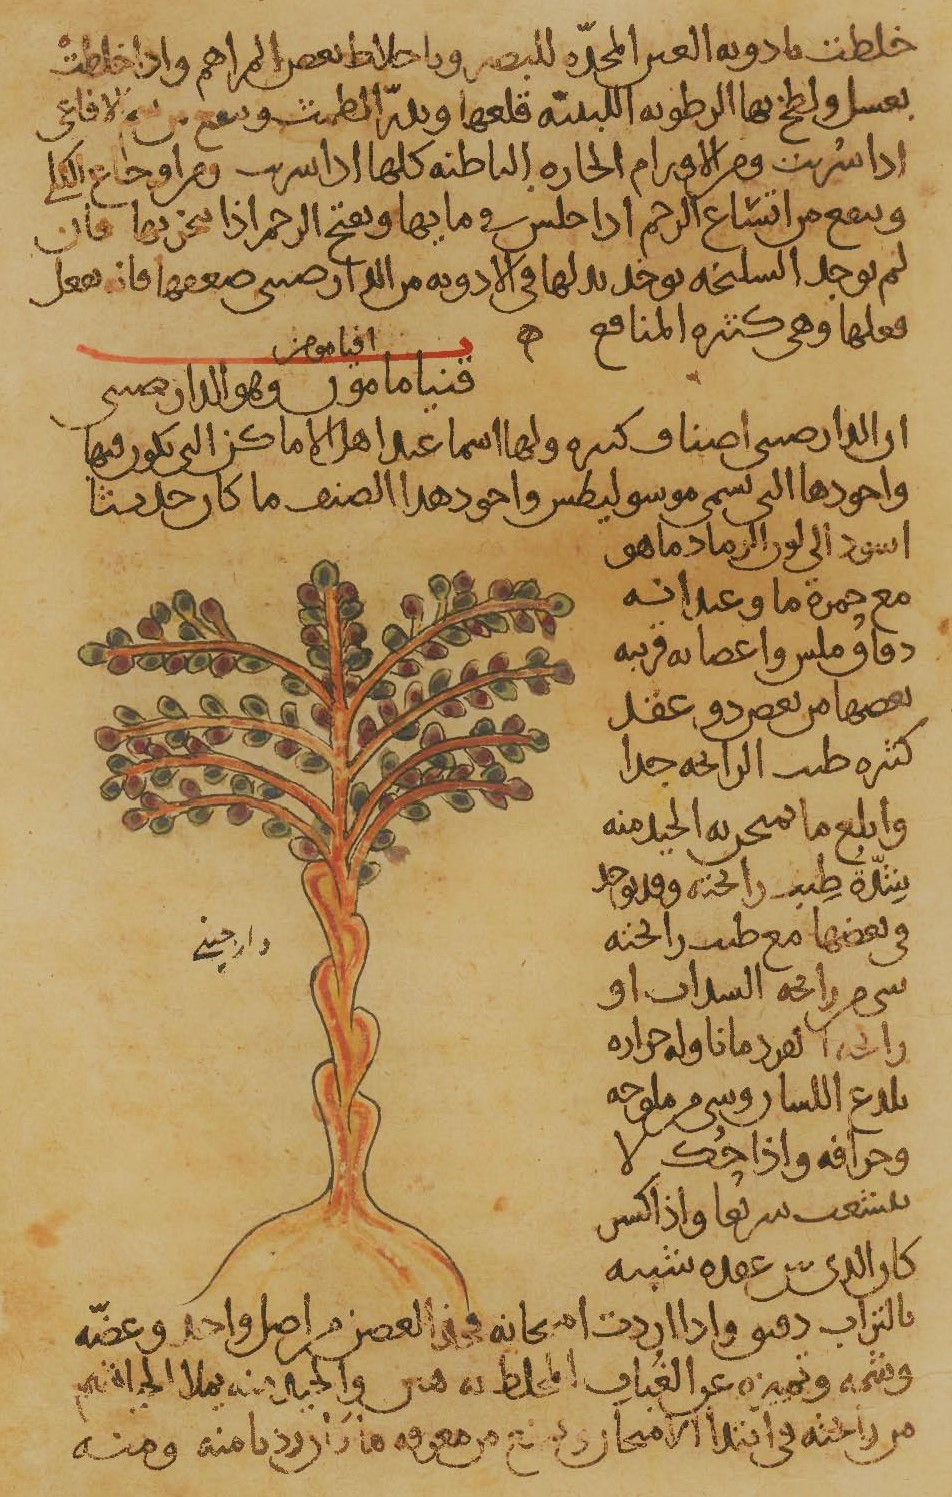
\includegraphics[width=0.5\textwidth]{imgs/figs/cinnamon_manuscipt_cr.jpg}
  \caption[Cinnamon tree in a \nth{10}-century Arabic manuscript.]{Cinnamon tree in a \nth{10}-century Arabic translation of Dioscorides's \gls{DMM}, a manuscript at the Oriental Collection of the University Library of Leiden (Shelfmark: Or. 289). This copy is from Samarkand, and dates to 1083, the time of the Karakhanids \parencite[f. 9a]{dioscorides_kitab_1083}}
\label{fig:cinnamon_manuscript}
\end{wrapfigure}

In the writings of Dioscorides from the \nth{1} century \AD{}, both classes of \gr{κινάμωμον} \textit{kinámōmon} and \gr{κασ(σ)ία} \textit{kas(s)ía} rind are listed, but he fails to mention their source \parencite{alam_darcini_2011}. Muslim writers translating the Greek works from the \nth{9} century rendered the classes as \textit{dārṣīnī} and \textit{salīkha} \parencite{alam_darcini_2011}. \Cref{fig:cinnamon_manuscript} shows a folio from a Greco-Islamic pharmacopoeia, where the heading right under the red stroke says: \ar{قينامامون وهو الدارصيني}
\textit{q\={i}n\={a}m\={a}m\={u}n wa-huwa l-d\={a}r\d{s}\={i}n\={i}} `\textit{Kīnāmāmon}, which is cinnamon', shows that Arabic translators transcribed the Greek names for herbal remedies, even when they had their own terminology. The Islamicate scholarly world of scholars were closely familiar with the Greek works, \textit{dārṣīnī} seems to have indicated the same category as Greek \textit{kinnámōmon}, and they knew a ``whole range of kinds'' of it.\footnote{For more on the Arabic transmission of Dioscorides's \textit{Materia medica}, see \textcite{gutas_arabic_2012}} Ibn al-Bayṭār (d. 1248), an Andalusian Arab physician, pharmacist, and botanist heavily relying on the writings of Dioscorides and Galen, listed the different kinds of cinnamon known under the category of \textit{dārṣīnī} in his \citetitle{ibn_al-baytar_kitab_1874}, citing Isḥāḳ b. Sulaymān \pvolcite[]{I/2}[p. 83, dārṣīnī]{ibn_al-baytar_kitab_1874}. \textcite{dietrich_dar_2004} introduces these products listed by Ibn al-Bayṭār: Chinese cinnamon \textit{dārṣīnī al-ṣīn} lit. `Chinese wood of China', an inferior kind called \textit{dār ṣūṣ}, the ``real cinnamon rind'' \textit{al-qirfa ʿalā l-ḥaqiqa}, the ``clove-rind'' \textit{qirfat al-qurunful} [sic], the ``pungent cinnamon'' \textit{al-ḥādd al-madhāq} lit. `the sharp of taste', etc. The term \textit{dārṣīnī} still exists in the Arabic scientific name for the genus \textit{Cinnamomum}, and as a colloquial term without an emphatic /s/; \ar{دارسين} (\textit{dārsīn}) in some Khalījī (Gulf) Arabic dialects, where the Persian influence was always strong.

According to \parencite{alam_darcini_2011}, some modern scholars have implied that ancient societies sourced their cinnamon from China overland, due to the interpretation of the name, but citing \textcite{laufer_sino-iranica_1919}'s \citetitle{laufer_sino-iranica_1919}, there is no Sinological evidence to support this. I agree with the author here that if cinnamon came from Asia, it must have arrived via the sea trade with South India and Lanka. Yūḥannā bin Māsūya (d. 955), a contemporary of al-Isrāʾīlī, mentioned three kinds of \textit{qirfa}: \textit{qirfat al-qaranful}, the best; \textit{qirfa} that smelled like camphor; and \textit{qirfa} that smelled like \textit{dārṣīnī} \parencite{alam_darcini_2011}.

Arabic names shown in \cref{table:names_cinnamon_ar}, similarly to English, focus geographical origin and genuineness, but also quality and grade. This shows us two things. First, people who were part of the spice trade and had some knowledge  on it were also concerned about the source of the \emph{real} cinnamon, not only the Europeans were actively trying to \emph{go} and find it some centuries later. Second, there must have been several sources of ``cinnamon''. It is not a secret that Arabia and neighboring East Africa had aromatic trees and shrubs, just think of myrrh and frankincense. It is not an impossible idea that words such as \textit{qirfa} and \textit{salīkha}---which literally meant `rind' or `bark' were sourced locally/regionally, and these terms were also applied to similar products arriving from Southeast Asia. As for \textit{dārsīnī}, it is without a doubt an eastern product. Terms, such as \textit{dārṣīnī al-ṣīn} [dārṣīnī of China/Chinese dārṣīnī] also indicate that it was a category, rather than a specific kind of product. 

\setlength{\tabcolsep}{2pt}

\begin{table}[!ht]
\centering
\begin{tabularx}{\textwidth}{@{}l>{\itshape \footnotesize}lr>{\itshape}lL>{\small}l@{}}
\toprule
\textbf{\#} & \multicolumn{1}{l}{\textbf{Species}} & \multicolumn{1}{l}{\textbf{Name}} & \multicolumn{1}{l}{\textbf{Tr.}} & \multicolumn{1}{l}{\textbf{Gloss}} & \multicolumn{1}{l}{\textbf{Source}} \\
\midrule
1	& Cinnamomum cassia	& دارصيني الدون	& dārṣīnī al-dūn	& inferior cinnamon	&  \\
2	& Cinnamomum cassia	& قرفة صينية	& qirfa ṣīnīyya 	& Chinese bark	& \textcite{wikipedia} \\
\textbf{3}	& \textbf{Cinnamomum cassia}	& \textbf{سليخة}	& \textbf{salīkha}	& \textbf{peel, strip}	& \textbf{\textcite{wehr_dictionary_1976}} \\
4	& Cinnamomum spp.	& الحاد المذاق	& al-ḥādd al-madhāq	& the sharp taste	& \textcite{dietrich_dar_2004} \\
5	& Cinnamomum spp.	& دارصيني	& dārṣīnī	& Chinese wood	& \textcite{dietrich_dar_2004} \\
6	& Cinnamomum spp.	& دارصيني الصين	& dārṣīnī al-ṣīn	& Chinese wood of China	& \textcite{dietrich_dar_2004} \\
\textbf{7}	& \textbf{Cinnamomum spp.}	& \textbf{قرفة}	& \textbf{qirfa}	& \textbf{bark, rind}	& \textbf{\textcite{wehr_dictionary_1976}} \\
8	& Cinnamomum spp.	& قرفة القرنفل	& qirfat al-qurunful	& the bark of clove	& \textcite{dietrich_dar_2004} \\
9	& Cinnamomum verum	& الدارصيني على الحقيقة	& al-dārṣīnī ʿalā l-ḥaqīqa	& the real darsini	& \textcite{dietrich_dar_2004} \\
10	& Cinnamomum verum	& القرفة على الحقيقة	& al-qirfa ʿalā l-ḥaqīqa	& the real bark	& \textcite{dietrich_dar_2004} \\
11	& Cinnamomum verum	& القرفة الأصلية	& al-qirfat al-aṣliyya	& the original bark	& \textcite{wikipedia} \\
12	& Cinnamomum verum	& القرفة السهيلانية	& al-qirfat al-sihīlānīya	& Sinhalese bark	& \textcite{alam_darcini_2011} \\
\bottomrule
\end{tabularx}
\caption{Various names for cinnamon in Arabic.}
\label{table:names_cinnamon_ar}
\end{table}



\setlength{\tabcolsep}{6pt}

\subsubsection{Chinese}
\label{sec:cinnamon_names_zh}

The Chinese language does not have two different words for cinnamon and cassia, the term 肉桂 \textit{ròuguì} [flesh-cinnamon] is used, referring to the `cassia bark' of \textit{C. cassia}, often just called ``Chinese cinnamon'' in English. Furthermore, one can come across \zh{桂皮} \textit{guìpí} [cinnamon-skin] `id.', and \textcite[399]{hu_food_2005} also lists \zh{官桂} \textit{guānguì} [official-cinnamon] `id.'. The latter makes sense if we imagine the resemblance of the curled barks of cinnamon to the written scrolls of the officials \parencite[see][732]{zhang_dictionary_2015}. \zh{桂心} \textit{guìxīn} [cinnamon-heart] `id.' refers to the inner bark specifically.\footnote{In case of some cassia varieties, the outer barks could be used as well.} Hu calls all these products---native to the mountainous regions of Vietnam and China borderlands---\textit{cassia}, and she reiterates the notion introduced by \parencite{ravindran_cinnamon_2004}, that Vietnamese and Chinese cassia is the same, explaining that those that are exported from Saigon are called \textit{Saigon cinnamon} in English, while the others transported to the south to Guangzhou and Hong Kong ``have the trade name \textit{cassia}'' \parencite[400]{hu_food_2005}. There is also \zh{桂枝} \textit{guìzhī} [cassia-branches] `cassia twigs', which is a particular kind of cinnamon product unique to \gls{TCM}, made up of the chopped up young branches of the cassia tree, and \zh{桂子} \textit{guìzǐ} [cassia-seeds] `cassia buds' referring to the fruits. As for the other cinnamon products found outside of China, medicinal products from \textit{C. burmannii} (root, bark, leaf), are called \zh{陰香} \textit{yīnxiāng} [yin-spice]\footnote{\textit{From the feminine, dark, ``negative'' half of the yin and yang concept.}} \parencite[179]{hu_enumeration_1999}.
if Sri Lankan cinnamon must be expressed, \zh{錫蘭肉桂} \textit{xīlánròuguì} `Ceylon cinnamon' is applicable, 

In historical texts the character \zh{桂} \textit{guì}\footnote{\textentry{CTP}{桂}---\url{https://ctext.org/dictionary.pl?if=en&char=\%E6\%A1\%82}} referred to cinnamon/cassia. The Sinogram of \textit{guì}, \gls{OC} /*kʷeːs/, is a phono-semantic compound made up of semantic \zh{木} `tree' + phonetic \zh{圭} \gls{OC} /*kʷeː/.
The first instance we are able to find in the corpus available in the \gls{CTP} of \textit{guì} is in the \gls{Liji}, from the Warring States period (\nth{5}c.--221 \BC{}):

\begin{quote}
    \tc{曾子曰:「喪有疾,食肉飲酒,必有草木之滋焉。以為姜桂之謂也。」 \\}Zeng-zi said, `When one during his mourning rites falls ill, and has to eat meat and drink spirits, there must be added the strengthening flavours from vegetables and trees;' meaning thereby ginger and cinnamon.\footnote{\gls{CTP}---\url{https://ctext.org/pre-qin-and-han?searchu=\%E6\%A1\%82}; translations from James Legge}
\end{quote}

Here too, we must be careful when identifying plants and plant products, because \textit{guì} can also be the sweet-scented osmanthus. In the past, \textit{guì} marked both cinnamon species from the laurel family (\textit{Lauraceae}), and sweet osmanthus (from Greek \textit{osme} `fragrant' and \textit{anthos}, `flower'), a fragrant flowering bush with tiny white flowers common all around East and mainland Southeast Asia, frequently found in city parks. Osmanthus (\taxonn{Osmanthus fragrans}{Lour.})---also called ``sweet olive'' and ``tea olive'' in English---is a species in the olive family \textit{Oleaceae} \parencite[191]{pearlstine_scent_2022}, and today it is referred to as \zh{桂花} \textit{guìhuā} [osmanthus-flower] to make a distinction. The synonym \zh{木犀} \textit{mùxi} is said to come from the similarity of the bark's striations and the rhinoceros's horn \parencite{chennault_reclusive_2006}; another name is \zh{九里香} \textit{jiǔlǐxiāng}, lit. `fragrant-for-nine-li'\footnote{\textit{Li} is an ancient measure of length, approximately equal to 500 meters.}. \textcite{chennault_reclusive_2006} uses reasoning along botanical lines, to find out if a line is about cinnamon or osmanthus. For example, if the \textit{guì}-wood is used for temple-building, it must be cinnamon (osmanthus is a shrub, less suitable for construction); if the verse talks about the scent of white or red flowers, it is likely to concern osmanthus (only the bark and leaves are aromatic in case of cinnamon, and cinnamon flowers are always white as opposed to osmanthus, where some varieties have orange/reddish flowers). Osmanthus is used to season tea and it is an ingredient in pastries. An alcoholic beverage called \textit{guihua} liquor also uses osmanthus tincture to flavor rice gin \parencite[627]{hu_food_2005}. Osmanthus flower is important in Chinese culture---from legends, in poetry, and as a Buddhist symbol---and it is associated with the Mid-autumn Festival. \textcite{chennault_reclusive_2006}'s essay on the identity of \textit{guì} explores the use of \textit{guì} in traditional---especially Buddhist---poetry, and clears the confusion between cinnamon and osmanthus in a Chinese literary context. The character \zh{桂} \textit{guì} appears in the \gls{Shuowen} and \gls{Kangxi} dictionaries, as well as the \gls{BCGM}, where it has been identified as \textit{Cinnamomum cassia} \parencite[732]{zhang_dictionary_2015}.

% Legend of osmanthus on the moon Chennault
% In BCGM
% Wu Gang 吳剛 [1] Mythological person, the immortal in the moon palace. According to the → You yang za zu 酉陽雜俎, he overindulged in his quest for immortality and was relegated to felling “moon cassia trees” (yue gui 月桂).

% \parencite{xiang_studies_2008}

Chinese names are concerned with plant parts first and foremost. Even the modern Chinese distinction between the two basic meanings of \textit{guì} (cinnamon/cassia and osmanthus) happens with the addition of other Chinese characters referring to the \textit{guì}'s meat or flesh (also used for fruit pulp) if it is cinnamon, or its flower if it is osmanthus. As a native spice of China, we will not find loanwords for cinnamon.

\begin{table}[!ht]
\centering
\begin{tabularx}{\textwidth}{@{}l>{\itshape \small}ll>{\itshape}lL>{\small}l@{}}
\toprule
\textbf{\#} & \multicolumn{1}{l}{\textbf{Species}} & \multicolumn{1}{l}{\textbf{Name}} & \multicolumn{1}{l}{\textbf{Tr.}} & \multicolumn{1}{l}{\textbf{Gloss}} & \multicolumn{1}{l}{\textbf{Source}} \\
\midrule
1	& Cinnamomum cassia	& \traditionalchinesefont{桂}	& guì	& cassia	& \textcite{defrancis_abc_2003} \\
2	& Cinnamomum cassia	& \traditionalchinesefont{桂皮}	& guìpí	& cassia-skin	& \textcite{defrancis_abc_2003} \\
3	& Cinnamomum cassia	& \traditionalchinesefont{桂心}	& guìxīn	& cassia-heart	& \textcite{hu_food_2005} \\
4	& Cinnamomum cassia	& \traditionalchinesefont{桂枝}	& guìzhī	& cassia-branches	& \textcite{hu_food_2005} \\
5	& Cinnamomum cassia	& \traditionalchinesefont{桂子}	& guìzǐ	& cassia-seeds	& \textcite{defrancis_abc_2003} \\
6	& Cinnamomum cassia	& \traditionalchinesefont{官桂}	& guānguì	& official-cassia	& \textcite{hu_food_2005} \\
\textbf{7}	& \textbf{Cinnamomum cassia}	& \textbf{\traditionalchinesefont{肉桂}}	& \textbf{ròuguì}	& \textbf{flesh-cassia}	& \textbf{\textcite{hu_food_2005}} \\
\textbf{8}	& \textbf{Cinnamomum verum}	& \textbf{\traditionalchinesefont{錫蘭肉桂}}	& \textbf{xīlán ròuguì}	& \textbf{Ceylon-flesh-cinnamon}	& \textbf{\textcite{wikipedia}} \\
\bottomrule
\end{tabularx}
\caption{Various names for cinnamon in Chinese.}
\label{table:names_cinnamon_zh}
\end{table}



\subsubsection{Summary}

\begin{table}[!ht]
    \caption{Conventionalized names for cinnamon in English, Arabic, and Chinese, found in dictionaries.}
\centering
\begin{tabularx}{\textwidth}{@{}ll>{\itshape}lLl>{\small}l@{}}
\toprule
\textbf{\#} & \textbf{Language} & \multicolumn{1}{l}{\textbf{Term}} & \textbf{Gloss} & \textbf{Loan} & \multicolumn{1}{l}{\textbf{Source}} \\
\midrule
1	& English	& bastard cinnamon	& 	& yes	& \textcite{oed} \\
2	& English	& cassia	& 	& yes	& \textcite{oed} \\
3	& English	& cinnamon	& 	& yes	& \textcite{oed} \\
\midrule
1	& Arabic	& salīkha	& peel, strip	& no	& \textcite{wehr_dictionary_1976} \\
2	& Arabic	& dārṣīnī	& Chinese wood	& yes	& \textcite{wehr_dictionary_1976} \\
3	& Arabic	& qirfa	& bark, rind	& no	& \textcite{wehr_dictionary_1976} \\
\midrule
1	& Chinese	& guì	& cassia	& no	& \textcite{defrancis_abc_2003} \\
2	& Chinese	& guìpí	& cassia-skin	& no	& \textcite{defrancis_abc_2003} \\
3	& Chinese	& guìzhī	& cassia-branches	& no	& \textcite{defrancis_abc_2003} \\
4	& Chinese	& guìzǐ	& cassia-seeds	& no	& \textcite{defrancis_abc_2003} \\
5	& Chinese	& ròuguì	& flesh-cassia	& no	& \textcite{defrancis_abc_2003} \\
\bottomrule
\end{tabularx}
\label{table:names_cinnamon}
\end{table}



To summarize, the two English quintessential names that cannot broken down into further parts in English---\textit{cinnamon} and \textit{cassia}---are both loanwords arriving on similar pathways, and also \glspl{wanderwort}. From the three Arabic words that play an important role here, two---\textit{qirfa} and \textit{salīkha}---are native Semitic words, while \textit{dārṣīnī} is a borrowing from Persian, which is the source language for many languages borrowing the name for cinnamon. As for Chinese, \textit{guì} is the original Sinogram for cinnamon, and all further words are compounded with this character. In \cref{table:names_cinnamon}, I listed the names that appear in modern dictionaries. One thing to notice here is that the further we are to the source of cinnamon and cassia geographically, the more likely it is for the name to be a loanword.




\subsection{The Contemporary Distribution of Spice Terms: The Case of Cinnamon}
\label{sec:case_of_cinnamon}

% Empirical Chapters
% Discuss and present your findings in a factual way.
% What are the results of your investigations?
% How do the findings relate to previous studies?
% Was there anything surprising or that didn’t work out as planned?
% Are there any themes or categories that emerge from the data?

This section aims to give an overview on the terminology used by various languages when referring to cinnamon. These words are connected to the spread of material culture, and a (not-so) specific plant product used and coveted for its aroma, used as spice and medicine. Known by humans for millennia, cinnamon is now present essentially on a global scale, and by exploring its names in multiple languages, we can reconstruct its linguistic genealogy. These results also tell a story; they tell us an account on the linguistic history of \emph{cinnamonic} words, their origins, diffusion, and ultimately, the story of cinnamon. We can infer information on the trade routes and the peoples who transmitted it, and identify the cultures that used and diffused knowledge on it. 

\begin{figure}[ht!]
    \centering
    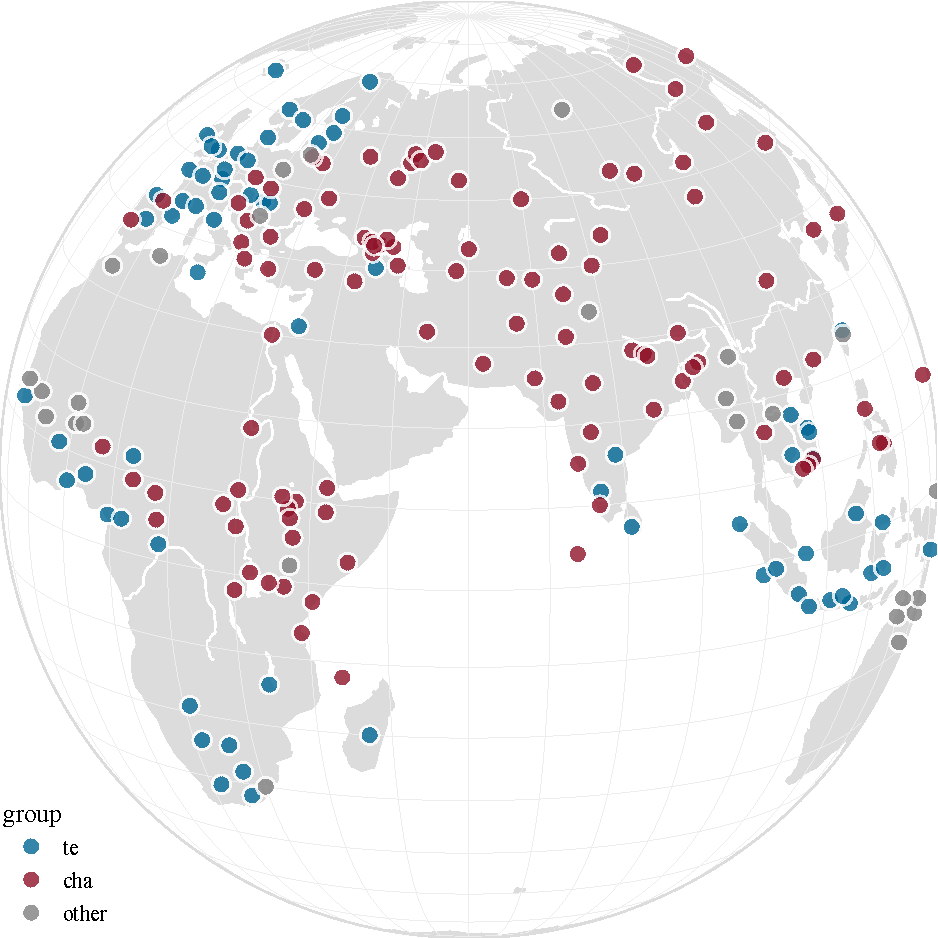
\includegraphics[width=\linewidth]{imgs/plots/distribution_tea.pdf}
    \caption[Distribution of words for tea from Sinitic \textit{cha} and Minnan \textit{te}.]{Distribution of words for tea from Sinitic \textit{cha} and Minnan \textit{te}, based on the data around the globe, from the \gls{WALS} dataset.}
    \label{fig:distribution_tea}
\end{figure}

To those of us who interested in the spread of words, especially \glspl{wanderwort} and their underlying cultural, historical, and geo-political significance, the map of tea might come to mind. This is a map that shows the journey of words for tea (either from Sinitic \textit{cha} or Minnan \textit{te}), and their distribution in a sample of the world's languages. The point of this map is that it clearly shows if the name for tea arrived by overland trade or via a sea route. This peculiar phenomenon is a feature on its own (138A) in \gls{WALS}, and have been described in a chapter by \textcite{dahl_tea_2013}.\footnote{The accompanying map is available online at \url{https://wals.info/feature/138A\#2/25.5/143.6}} Discussions and maps of the land vs. sea distribution of tea terminology have since made it into popular science magazines and articles, made rounds on Twitter, and hence relatively well known.\footnote{See for example \textcite{sonnad_tea_2018} in Quartz: \url{https://qz.com/1176962/map-how-the-word-tea-spread-over-land-and-sea-to-conquer-the-world/} or \textcite{netchev_movement_2022} in the World History Encyclopaedia: \url{https://www.worldhistory.org/image/14112/movement-of-tea--cha-around-the-globe/}} On a more scientific note, the distribution of tea words are discussed in detail by \autocite[261-270]{mair_true_2009} in an appendix titled \textit{A Genealogy of Words for Tea}, with including a discussion on historical phonology.

Cinnamon as a spice is relatively common around the world, and the history of its diffusion goes back to thousands of years, with words attested as early as the Bible itself, as it was discussed in \cref{sec:cinnamon}. This is in contrast with the story of tea, in the sense that the international spread of tea is a relatively recent process in the economic history of plant products and colonial powers, and so we have a much clearer picture on the exact ways it was transmitted. Although tea-drinking in its homeland was practiced from time immemorial, and trade allowed it to spread regionally on networks, such as the Tea Horse Road, its present global domination is a result of \nth{17}-century European fascination and large scale shipping. While the tea map illustrates the long haul trade connections of the time, such as those between Europe and the Far East, the map of cinnamon shows traces of an older, more gradual spread that happened in stages, outlining a more geographically contiguous development, and incremental trade networks. The propagation of cinnamonic \glspl{wanderwort} mirrors the historical processes, and just as the story of cinnamon, the words' origins are sometimes obscured by the sheer time-depth that is covered.

\subsubsection{Methods}

Informative geospatial visualizations such as \cref{fig:distribution_tea} above are a powerful tool in conveying the information about spread and distribution of words, and they can also help us to notice patterns and connections faster and easier than studying long tables of words, especially when the distributions are more complex than the somewhat neat duality of tea. In this case study, I will attempt a classification for the words for cinnamon by looking at clusters and categorizing them according to their source, to see what the distribution of names today can tell us about the spread and history of cinnamon.

Because words for cinnamon or other spices are not included as features in balanced typological datasets, such as \gls{WALS} (tea is an exceptional feature in this database), I have attempted a manual collection of words for cinnamon based on dictionary entries. As a starting point, I have crawled data from the Wiktionary (\url{https://en.wiktionary.org}), which is the closest resource we currently have to an open- and crowd-sourced multilingual dictionary. Similarly to the Wikipedia, the Wiktionary is edited and reviewed by the community, which has both advantages and disadvantages. On one hand, information on the Wiktionary is free, broad in scope, it usually represents the public consensus, and often well cited. On the other hand, it is not always complete, the available languages do not represent a balanced sample from a typological point of view, and the information can sometimes be ill-informed or deprecated. In any case it is a rich resource to start with. 

For cinnamon, first I scraped the translations for the word \textit{cinnamon} in the sense `spice' \autocite{wiktionary_cinnamon_nodate}, and cleaned the data using regular expressions. After this, I have performed a round of manual checking where I fixed obvious mistakes in word forms and transliterations by consulting other dictionaries and reference works, in the languages and scripts I felt competent to do so. I proceeded to add a few missing translations with the help of other lexicographical resources and the Google Neural Machine Translation engine's Python API \autocite{wu_googles_2016}.\footnote{\url{https://pypi.org/project/googletrans/}} Then, I analyzed each word in terms of etymological origin, and assigned them to categories. For example, words derived from Greek \textit{kinnámōmon}, such as Lithuanian \textit{cinamonas} or English \textit{cinnamon} constitute one category, and words derived from Persian \textit{dârčin}, such as Turkish \textit{tarçın} or Hindi \textit{dālcīnī}, make up another. I continued this categorization for all instances, and created a new category for every group that has at least three attested members. Instances that do not belong to any group or undetermined were assigned to ``other''. Finally, I merged this dataset with language data obtained from the databases of both \gls{WALS} \autocite{dryer_wals_2013} and Glottolog \autocite{hammarstrom_glottolog_2022} to prepare for geospatial plotting. The datasets were handled using the \texttt{pandas} library in Python, and the visualizations were created using the \texttt{plotly} Python library \autocites{pandas, plotly}.

\subsubsection{Results}

\Cref{fig:distribution_cinnamon} shows the results of the analysis above, on a geographical scatter plot. As it can be seen, there are six groups in total: canela, kinnamon, korica, qirfa, darchin, and gui, with a seventh one---other---containing those that do not belong to any of these. It is also noticeable that the groups that were manually identified form geographical clusters, for example, the gui group appears in East Asia, while the canela group is mainly found in Europe. Lastly, I would like to draw attention that the ``other'' group has a high number of members in regions where cinnamon (or cassia) is native. The canela group represent words that derived from Latin, the kinnamon group contains words going back to Greek, and the korica group represent mostly Slavic languages. Qirfa words are derived from Arabic, darchin gathers terms from the Persianate world, and gui embraces some terms from the Sinosphere. Let us now look at these categories one by one.

\begin{figure}[!ht]
    \centering
    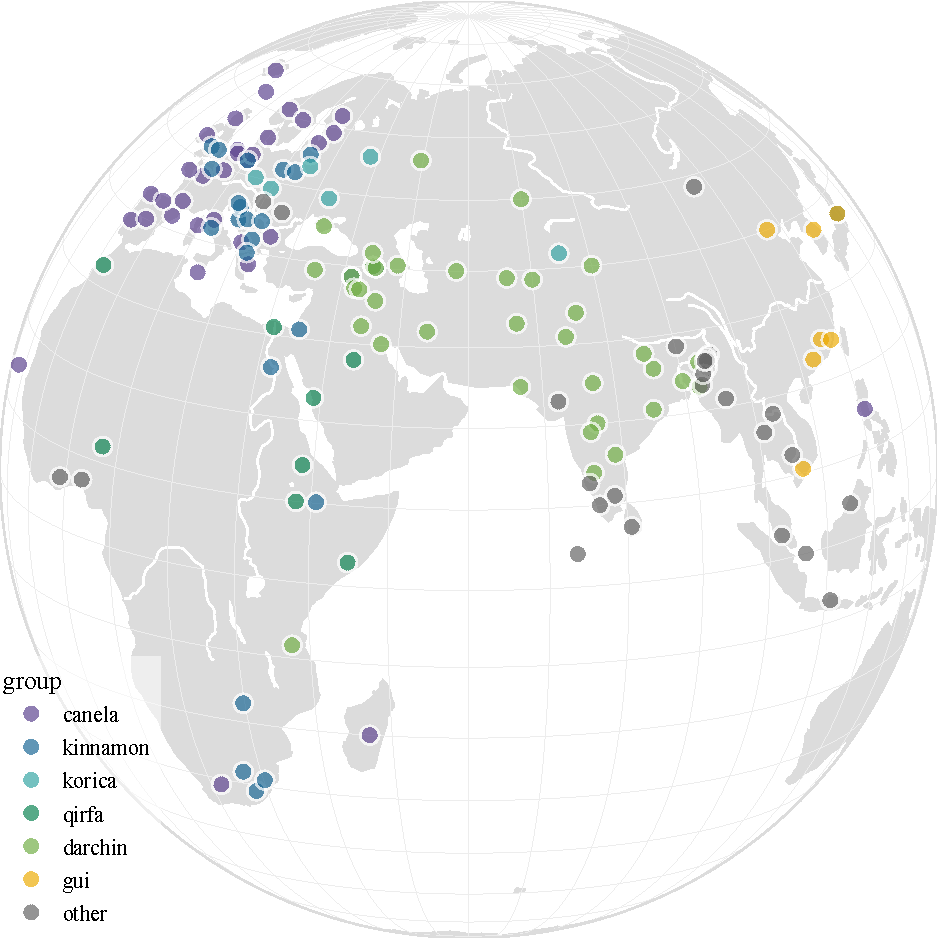
\includegraphics[width=\linewidth]{imgs/plots/distribution_cinnamon.pdf}
    \caption[Distribution of words for cinnamon in a few languages around the globe.]{Distribution of words for cinnamon in a few languages around the globe. For a full, interactive and explorable version of the plot, please visit the following link: \url{http://htmlpreview.github.io/?https://github.com/partigabor/phd-thesis-viz/blob/main/distribution_cinnamon.html}}
    \label{fig:distribution_cinnamon}
\end{figure}

\begin{note}
 The interactive plot can be rotated, zoomed in and out, and the groups of data points can be isolated with a double-click on the group name/icon. Hovering over a data point will bring forward further information on the term, its transliteration, associated language and language family.
\end{note}

\subsubsection{The canela group}

Words belonging to this group are cognates of Spanish \textit{canela} and its variants in Romance languages, which have been formed with the diminutive of Latin \textit{canna} `reed, cane'. It is named so after the curled shape of the cinnamon sticks resembling a little, hollow reed-pipe.\footcite[cannel]{oed} Latin \textit{canna} itself is a loanword from Greek \gr{κᾰ́ννᾱ}
\textit{kánna} `reed, pole', which is probably a borrowing from a Semitic language (cf. Arabic \ar{قناة}
\textit{qan\={a}h} `hollow spear, cane; conduit, canal', Hebrew \he{קָנֶה}
\textit{qāneh} `stalk, reed, cane', Aramaic \sy{ܩܢܝܐ} 
\textit{qanyā} `id.'\footnote{\url{https://cal.huc.edu/oneentry.php?lemma=qnh+N&cits=all}}).\footcite[cane]{OED} According to \textcite[636]{beekes_etymological_2010} the Greek word is from ``Babylonian-Assyrian'' (Akkadian) \cu{\GA\NU\UU\UM} \textit{qanû} `reed', which may come from ``Sumerian-Akkadian'' (Sumerian) \cu{\GI} \textit{gin} `id.' \pvolcite[cf.]{13}[85]{roth_assyrian_2004}, and proceeds to give Ugaritic \textit{qn} and Punic \textit{qn'} as further Semitic attestations.

The distribution of this group is overwhelming in Europe, which seems to echo the strong influence of Latin vocabulary, especially in the developing Romance languages. One example would be Old French \textit{canele} (modern \textit{cannelle}), which was formed within French from \textit{canne} `cane', and first attested in the first half of the \nth{12} century from an epic poem describing a fictional expedition of Charlemagne to Jerusalem\footnote{\textit{Le Pèlerinage de Charlemagne [The Pilgrimage of Charlemagne]}, or \textit{Voyage de Charlemagne à Jérusalem et à Constantinople [Charlemagne's Voyage to Jerusalem and Constantinople]}, (c. 1140).}, and the local vendors selling cinnamon, pepper, and ``other fine spices''.\footcite[cannelle \link{https://www.cnrtl.fr/definition/cannelle}]{tlfi}. The \gls{TLFi} explains that this word exists in most romance languages and it is impossible to determine its progress, and also notes that the medieval Latin is not attested in the `cinnamon' sense. Either French or Italian was the usual donor for other European languages, take for example Dutch \textit{kaneel}, or Finnish \textit{kaneli} through Swedish \textit{kanel}. Spanish \textit{canela} is attested around 1250, from ``Italian'' (Medieval Latin) \textit{cannella} \autocites[125]{corominas_breve_1987}[98]{gomez_de_silva_elseviers_1985}. Due to later colonization by European powers, many of these terms spread elsewhere, e.g.: Tagalog \textit{kanela} from Spanish, or Haitian Creole \textit{kannèl}.

\textit{\obs Cannel}, also earlier as \textit{canel} had entered English usage in the \nth{13} century from French, but is now obsolete. It existed in Early Modern English up until the \nth{18} century, and was gradually replaced by \textit{cinnamon} (also arriving through French), which was first attested in the first half of the \nth{15} century (see Etymology \ref{ety:cinnamon}). Neo Latin \textit{canella} also appeared for a brief time, but its meaning as `cinnamon' waned, and now it is used in botany to refer to a plant genus.

In many other languages of Europe the opposite happened, and an existing word from Greek was replaced by the Latin term. Even Modern Greek uses \textit{kanéla}, re(?)-borrowed from Italian \textit{cannella}, instead of the Ancient Greek \textit{kinnámōmon}. 

\subsubsection{The kinnamon group}

This group centers around Ancient Greek \textit{kinnámōmon}, most possibly a loanword from a Semitic language as I discussed in \cref{sec:cinnamon_names_en}. \textit{Kinnámōmon} is the source of words for cinnamon in many European languages (e.g.: German \textit{Zimt}, Lithuanian \textit{cinamonas}, and English \textit{cinnamon}), prominently in Central Europe and the Middle East. In most cases, these words represent an area where words derived from Latin cannella (or one of its descendants) did not replace the earlier word derived of \textit{kinnámōmon}. This group also contains South Slavic languages in the Balkan linguistic area (e.g.,Slovenian \textit{cimet}, Serbian \cy{цимет} \textit{cimet}) where it arrived via the earlier German term \textit{Zimmet} (now \textit{Zimt}), and therefore it diverges from West and East Slavic branches for this lexical item. It reached Southeast Europe in the \nth{16} century \autocite[cimet]{snoj_slovenski_1997}\footnote{Fran---\url{https://fran.si/193/marko-snoj-slovenski-etimoloski-slovar/4285437/cimet?View=1\&Query=cimet}}, from which we can assume that cinnamon started to arrived here from the West during this turbulent time in the Balkans, in the middle of the Ottoman Empire's European expansion.

\subsubsection{The korica group}

The korica group contains languages that use words derived from the inherited Slavic lexicon, in this case the East and West Slavic branches. Proto-Slavic \textit{*korica} `bark' is a derivative of \textit{*korà} `bark',\footnote{\gls{PIE} \textit{*(s)kor-} `to cut'}\footcite[]{derksen_etymological_2008} the suffix \textit{-ica} is diminutive. Old Church Slavic \textit{koricę} meant `cinnamon', and further cognates are Russian \textit{koríca} `id.', Ukrainian \cy{кори́ця} \textit{korýcja} `id.' (East Slavic), Czech \textit{skořice} `id.' (West Slavic). In other cases, words derived from \textit{*korica} can mean `bark, crust' (e.g.,Serb-Croatian) or `cover (of a book), binding' (e.g.,Bulgarian) \autocite[235]{derksen_etymological_2008}. Due to the influence of Russian during Soviet times, some Central Asian Turkic languages ended up with foreign words in their vocabularies, e.g.,Kirghiz \cy{корица} \textit{korica}.

\subsubsection{The qirfa group}

The qirfa group contains languages from Africa and the Middle East, whose words for cinnamon were borrowed from Arabic \textit{qirfa}, for example Hausa \textit{kirfa} \autocite[114]{newman_hausa-english_2007} and Amharic \am{ቀረፋ} \textit{qäräfa} \autocite[74]{leslau_concise_1996}.

\subsubsection{The darchin group}

Names for cinnamon in this category originate from Persian, as it was explained in \cref{sec:cinnamon_names_ar}. According to the data this cluster has the largest geographical extent, and by number of instances constitutes the largest group, almost head to head with the group of canela. Darchin represents the earliest stage of cinnamon's westward spread from South, Southeast, or East Asia, depending which cinnamon or cassia we think became the first cinnamon of commerce. Consulting the plot we can witness the huge influence Persian had in this step of transmission to the Middle East and Central Asia. We can also see that central and north Indian languages use a loanword from Persian, which can be explained by the Persianate\footnote{For a discussion on this term, see \textcite{green_persianate_2019}.} societies that resulted from the Islamic conquest of India, starting from the \nth{13} century. The first sultan to ravage the land, Mahmud of Ghazni was a Persianized \textit{mamluk} Turk, who laid the foundations with his raids in the \nth{11} century for a series of Muslim dynasties on the Indian subcontinent, culminating in the Mughal Empire (1526–1857) and what we define today as Indo-Persian culture \autocite[33]{eaton_india_2019}.

\subsubsection{The gui group}

The gui group contains terms from the Sinosphere, words that borrowed the Sinogram \zh{桂} \textit{gui} (see \cref{sec:cinnamon_names_zh}), such as Japanese \jp{桂} \textit{kei} `cinnamon or cassia tree', synonym with \jp{肉桂 (肉桂)} \textit{nikkei}, Korean \ko{계} \textit{gye} as \ko{계피 (桂皮)} \textit{gyepi} and \ko{육계 (肉桂)} and the Sino-Vietnamese \vi{quế}. This shows that the Chinese transmitted their cassia to their immediate neighbors East and Southwest, together with the word and character for it. However, there is little evidence for trade in cinnamon between China and Southeast Asia in early history, \textcite{wang_nanhai_1958} does not give any information on it in his \citetitle*{wang_nanhai_1958}. \autocite{wang_nanhai_1958} This makes sense if we remember that all regions active in the South China Sea maritime trade---from Guangdong to Sumatra to Lanka---had their own source of cinnamon, and traders would only transport it westwards.

\subsubsection{Others}

We can see that the category of ``other'' is prevalent in areas where cinnamon of various kinds is native and therefore these languages often have native words to refer to it. Many words from these group are derived from the meaning of `tree bark, skin, peel' Malay/Indonesian \textit{kulit kayu manis} [bark-wood-sweet] `sweet wood bark', where \textit{kulit} `skin, bark' is often omitted, or Dhivehi \textit{fonithoshi} [sweet-bark]. Hungarian \textit{fahéj} [tree-bark] is made by compounding and was attested in ca. 1395 \autocite[fahéj]{zaicz_etimologiai_2006}, Romanian \textit{scorțișoară}\footnote{Diminutive of \textit{scoarță} `bark', from Latin \textit{scortum} `hide, skin', \gls{PIE} *(s)ker- `to cut'.}, is perhaps modeled after Slavic \textit{*korica}.

\subsubsection{Conclusion}

So what does this tell us exactly? It shows that the modern state of spice terms' distribution is neatly arranged according to the influential languages that spread the name for particular material, pointing to certain civilizations who used, traded, and carried it, and had great influence over their neighbors. In the future, I hope to extend this approach to other spices, as it would be fascinating to compare the data of many different items and their distribution patterns.

















%--------------------------------------------
% EE:
% XV. ME. sinamome — (O)F. cinnamome — L. cinnamōmum — Gr. kinnámōmon; later refash. after L. cinnamon, -um — Gr. kínnamon, of Sem. orig. (cf. Heb. ḳinnāmōn).

% OEymonline:
% cinnamon (n.)
% spice obtained from the dried inner bark of a tree in the avocado family, late 14c., from Old French cinnamone (13c.), from Latin cinnamum, cinnamomum "cinnamon" (also used as a term of endearment), from Greek kinnamomon, from a Phoenician word akin to Hebrew qinnamon (with ending altered in Greek by folk-etymology). Ceylon cinnamon, the true cinnamon, is used in Britain, but American cinnamon is almost always from the related cassia tree of Southeast Asia and is stronger and sweeter. As an adjective, "of the color of cinnamon, light reddish-brown," 1680s. Related: Cinnamic.

% MW:
% Middle English cynamone, cynamum, from Middle French \& Latin; Middle French cinnamome, from Latin cinnamomum, cinnamon, cinnamum, from Greek kinnamōmon, kinnamon, of non-Indo-European origin; akin to Hebrew qinnāmōn cinnamon
% First Known Use: 14th century (sense 1c)

% AH:
% [Middle English cinamome, from Old French, from Latin cinnamōmum, from Greek kinnamōmon, probably of Semitic origin; akin to Hebrew qinnāmôn.]

% Wiktionary:
% From Middle English synamome, from Old French cinnamone, from Latin cinnamon, cinnamōmum, from Ancient Greek κιννάμωμον (kinnámōmon), later κίνναμον (kínnamon), probably to be explained as “Chinese amomum”, ἄμωμον (ámōmon) being, only cognate to Classical Syriac ܚܡܵܡܵܐ (ḥəmāmā) and Arabic حَمَامَا (ḥamāmā), a phytonym of lost provenience for a varied genus Amomum of spice and drug plants; compare for this composition the Iranian designation دارچین (dârčin, literally “Chinese tree”). 



% EE:
% kind of cinnamon. OE. and ME., but not naturalized till XVI. — L. cas(s)ia — Gr. kasíā — Heb. ḳeṣīʾh bark resembling cinnamon, f. ḳāṣāʾ strip off.

% OE:
% cinnamon-like plant of tropical regions, late Old English, from Latin cassia, from Greek kasia, from Hebrew q'tsi-ah "cassia," from qatsa "to cut off, strip off bark."

% MW:
% Middle English, from Old English, from Latin casia, cassia, from Greek kasia, kassia, of Semitic origin; akin to Hebrew qĕṣīʽāh cassia
% First Known Use: before 12th century (sense 1)

% AH:
% [Middle English, from Latin casia, cassia, aromatic tree of the genus Cinnamomum, from Greek kasiā, kassiā, probably of Phoenician origin; akin to Hebrew qəṣīyâ, tree of the genus Cinnamomum yielding a spice inferior to cinnamon, probably ultimately of Chinese origin.]

% WK:
% From Latin cassia (“cinnamon”), from Ancient Greek κασσία, κασία, κάσια (kassía, kasía, kásia), from Hebrew קְצִיעָה (qəṣīʿā), from Aramaic קְצִיעֲתָא (qəṣīʿătā), from קְצַע (qṣaʿ, “to cut off”). Compare Kezia. 

% ETYM An oriental loanword; cf. Hebr. qe tah, Assyr. kasia. Originally Austro-Asiatic ???